% !TeX spellcheck = en_GB

%%%%%%%%%%%%%%%%%%%%%%%%%%%%%%%%%%%%%%%%%%
%                                        %
%    Engineer thesis LaTeX template      % 
%                                        %
%%%%%%%%%%%%%%%%%%%%%%%%%%%%%%%%%%%%%%%%%%



\documentclass[a4paper,twoside,12pt]{book}
\usepackage[utf8]{inputenc}                                      
\usepackage[T1]{fontenc}  
\usepackage{amsmath,amsfonts,amssymb,amsthm}
% \usepackage[polish,british]{babel} 
\usepackage{indentfirst}
\usepackage{lmodern}
\usepackage{graphicx}
\usepackage{subcaption}
\captionsetup{compatibility=false}
\usepackage{float}
\usepackage{hyperref}
\usepackage{booktabs}
\usepackage{tikz}
\usepackage{pgfplots}
\usepackage{mathtools}
\usepackage{geometry}
\usepackage[page]{appendix} 
\usepackage[backend=bibtex]{biblatex}
\addbibresource{thebibliography.bib}

\usepackage{setspace}
\onehalfspacing


\frenchspacing

\usepackage{listings}
\lstset{
	language={},
	basicstyle=\ttfamily,
	keywordstyle=\lst@ifdisplaystyle\color{blue}\fi,
	commentstyle=\color{gray}
}

% Helps when line is to wide and can't be broken properly
\setlength{\emergencystretch}{10pt}
%%%%%%%%%

 

%%%%%%%%%%%% FANCY HEADERS %%%%%%%%%%%%%%%

\usepackage{fancyhdr}
\pagestyle{fancy}
\fancyhf{}
\fancyhead[LO]{\nouppercase{\it\rightmark}}
\fancyhead[RE]{\nouppercase{\it\leftmark}}
\fancyhead[LE,RO]{\it\thepage}
\setlength{\headheight}{15pt}% at least 14.49998pt


\fancypagestyle{onlyPageNumbers}{%
   \fancyhf{} 
   \fancyhead[LE,RO]{\it\thepage}
}

\fancypagestyle{PageNumbersChapterTitles}{%
   \fancyhf{} 
   \fancyhead[LO]{\nouppercase{\it\rightmark}}
   \fancyhead[RE]{\nouppercase{\it\leftmark}}
   \fancyhead[LE,RO]{\it\thepage}
}


%%%%%%%%%%%%%%%%%%%%%%%%%%%
% listings 
\usepackage{listings}
\lstset{%
language=C++,%
% commentstyle=\textit,%
% identifierstyle=\textsf,%
% keywordstyle=\sffamily\bfseries, %\texttt, %
% basicstyle=\small,%
basicstyle=\fontsize{11}{13}\selectfont\ttfamily,%
commentstyle=\itshape\color{purple!40!black},%
identifierstyle=\color{blue},%
keywordstyle=\bfseries\color{green!40!black},%
stringstyle=\color{orange},
%captionpos=b,%
tabsize=3,%
frame=lines,%
numbers=left,%
numberstyle=\tiny,%
numbersep=5pt,%
breaklines=true,%
morekeywords={uint8_t, uint16_t, uint32_t, int8_t, int16_t, int32_t, float32_t, __attribute__, section, aligned},%
escapeinside={@*}{*@},%
texcl=true, % wylacza tryb verbatim w komentarzach jednolinijkowych
}
%%%%%%%%%%%%%%%%%%%%%%%%%%%%%%%%%%%%

% % %%%% TODO LIST GENERATOR %%%%%%%%%

% % \usepackage{color}
% % \definecolor{brickred}      {cmyk}{0   , 0.89, 0.94, 0.28}

% % \makeatletter \newcommand \kslistofremarks{\section*{Remarks} \@starttoc{rks}}
% %   \newcommand\l@uwagas[2]
% %     {\par\noindent \textbf{#2:} %\parbox{10cm}
% % {#1}\par} \makeatother


% % \newcommand{\remark}[1]{%
% % {%\marginpar{\textdbend}
% % {\color{brickred}{[#1]}}}%
% % \addcontentsline{rks}{uwagas}{\protect{#1}}%
% % }

% % %%%%%%%%%%%%%% END OF TODO LIST GENERATOR %%%%%%%%%%% 

% % % some issues...

\newcounter{PagesWithoutNumbers}

\newcommand{\hcancel}[1]{%
    \tikz[baseline=(tocancel.base)]{
        \node[inner sep=0pt,outer sep=0pt] (tocancel) {#1};
        \draw[red] (tocancel.south west) -- (tocancel.north east);
    }%
}%

\newcommand{\MonthName}{%
  \ifcase\the\month
  \or January% 1
  \or February% 2
  \or March% 3
  \or April% 4
  \or May% 5
  \or June% 6
  \or July% 7
  \or August% 8
  \or September% 9
  \or October% 10
  \or November% 11
  \or December% 12
  \fi}


%%%%%%%%%%%%%%%%%%%%%%%%%%%%%%%%%%%%%%%%%%%%%%
% Helvetica font macros for the title page:
\newcommand{\headerfont}{\fontfamily{phv}\fontsize{18}{18}\bfseries\scshape\selectfont}
\newcommand{\titlefont}{\fontfamily{phv}\fontsize{18}{18}\selectfont}
\newcommand{\otherfont}{\fontfamily{phv}\fontsize{14}{14}\selectfont}

%%%%%%%%%%%%%%%%%%%%%%%%%%%%%%%%%%%%%%%%%%%%%%
%%%%%%%%%%%%%%%%%%%%%%%%%%%%%%%%%%%%%%%%%%%%%%
%%%%%%%%%%%%%%%%%%%%%%%%%%%%%%%%%%%%%%%%%%%%%%
%%%%%%%%%%%%%%%%%%%%%%%%%%%%%%%%%%%%%%%%%%%%%%
%%%%%%%%%%%%%%%%%%%%%%%%%%%%%%%%%%%%%%%%%%%%%%
%%%%%%%%%%%%%%%%%%%%%%%%%%%%%%%%%%%%%%%%%%%%%%
%%%%%%%%%%%%%%%%%%%%%%%%%%%%%%%%%%%%%%%%%%%%%%


\newcommand{\Author}{Michał Mieszczak}
\newcommand{\Supervisor}{dr inż. Jerzy Fiołka}
\newcommand{\Consultant}{Name Surname, PhD}
\newcommand{\Title}{Realization of digital audio effects on high-performance MCU platform.}
\newcommand{\Polsl}{Silesian University of Technology}
\newcommand{\Faculty}{Faculty of Automatic Control, Electronics and Computer Science}


% Deals with some compatibility warning
\pgfplotsset{compat=1.16}

\begin{document} 
	
%%%%%%%%%%%%%%%%%%  Title page %%%%%%%%%%%%%%%%%%% 
\pagestyle{empty}
{
	\newgeometry{top=2.5cm,%
	             bottom=2.5cm,%
	             left=3cm,
	             right=2.5cm}
	\sffamily
	\rule{0cm}{0cm}
	
	\begin{center}
	
\includegraphics[width=29mm]{polsl}
	\end{center} 
	\vspace{1cm}
	\begin{center}
	\headerfont \Polsl
	\end{center}
	\begin{center}
	\headerfont \Faculty
	\end{center}
	\vfill
	\begin{center}
	\titlefont Engineer  thesis
	\end{center}
	\vfill
	
	\begin{center}
	\otherfont \Title\par
	\end{center}
	
	\vfill
	
	\vfill
	 
	\noindent\vbox
	{
		\hbox{\otherfont Author: \Author}
		\vspace{12pt}
		\hbox{\otherfont Supervisor: \Supervisor}
		% \vspace{12pt}
		% \hbox{\otherfont consultant: \Consultant}
	}
	\vfill 
 
   \begin{center}
   \otherfont Gliwice,  \MonthName\ \the\year
   \end{center}	
   \restoregeometry
}
  

\cleardoublepage
 
\rmfamily
\normalfont

%%%%%%%%%%%%%%%%%% Table of contents %%%%%%%%%%%%%%%%%%%%%%
\pagenumbering{Roman}
\pagestyle{onlyPageNumbers}
\tableofcontents

%%%%%%%%%%%%%%%%%%%%%%%%%%%%%%%%%%%%%%%%%%%%%%%%%%%%%
\setcounter{PagesWithoutNumbers}{\value{page}}
\mainmatter
\pagestyle{PageNumbersChapterTitles}



\chapter{Introduction}\label{ch:intro}
The rapid development of technology lead to the moment,
when anybody can afford a development board.
There are literally thousands of different choices
covering wide spectrum of applications and price ranges.
Learning how to program microcontrollers without leaving a house
has became possible thanks to evolution of the internet.
Hundreds of websites provide tutorials devoted to
many topics and aspects of embedded technology,
which are addressed to beginners as well as 
experienced developers.

Hobbysts all around the world create products for different applications,
that can easily compete with their professional counterparts in both price and quality.

One example of such a field is market of sound related equipment.
More and more small companies are growing out of nowhere,
providing butique studio recording and processing equipment
with great customer service and support.




\chapter{Goals and tasks of the project}\label{ch:goals}
The main goal of the project is to develop an extention to existing development board,
which uses a modern, high-performance microcontroller.
The device should process stereo audio signal to achieve a selection of different effects
while delivering decent sound quality.
Following tasks are required to finish the project:

\begin{enumerate}
    \item Choice of components
    \begin{itemize}
        \item evaluation board
        \item operational amplifiers
        \item additional devices
    \end{itemize}

    \item List of features
    \begin{itemize}
        \item list of audio effects
        \item user interface
    \end{itemize}

    \item Creating the physical layer of device
    \begin{itemize}
        \item block diagram
        \item schematic
        \item PCB
        \item assembly 
    \end{itemize}

    \item Developing software
    \begin{itemize}
        \item choosing programming language
        \item choosing IDE, text editor, toolchain and frameworks
        \item writing and testing the program (user interface, effects)
    \end{itemize}
\end{enumerate}




\chapter{Topic analysis}\label{ch:analysis}
This chapter is devoted to main concerns related to the project,
that need to be considered at the beginning.
These will determine all important features and parameters of the device.

\section{Data acquisition}
The nature of audio signal is analog. This means,
that it should be conditioned in a proper way before it can be processed by digital circuitry.
It is done by ADC and coresponding preamplifier.

Signal must be reduced from continuous-time to discrete-time.
This process is called sampling and requires reading value of the signal in equal intervals of time.
Range of audible frequencies is considered to be 20Hz to 20kHz
and we need the whole range to acheive reasonable quality.
According to the concept of Nyquist frequency, the sampling frequency should be at least
twice as high as maximum frequency present in the signal.
In case of audio signal, it must be at least 40kHz.
There are some typical sampling frequencies preffered for audio signals such as: 44,1kHz, 48kHz,
96kHz, 192kHz and it would be a good idea to use one of them.

Furthermore ADC quantizes the value of the signal.
This means, that signal can take one of finite number of values.
The count of possible values is equal to \(2^n\), where n is the bit depth of the converter.

As stereo signal consists of two separate channels,
there sould be two identical sets of preaplifiers and converters.

\section{Output generation}
Processed digital signal must be converted back to analog.
This is done using DAC and corresponding amplifier.
DAC converts digital value into specific analog voltage,
outputs it and holds the value until succesive sample is to be outputted.
The figure \ref{fig:sine} shows an example of sinusoidal
function generated by a DAC.

\begin{figure}[H]
    \centering
    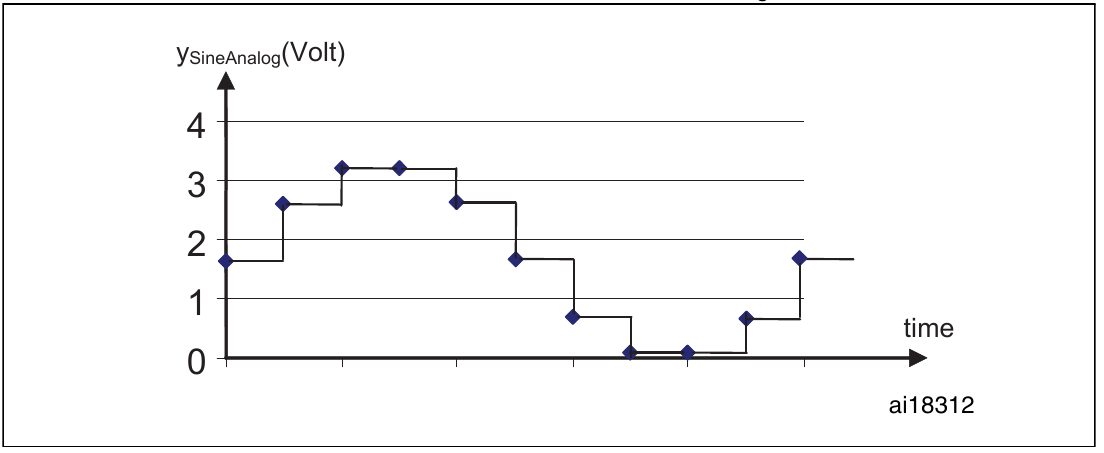
\includegraphics[width=\textwidth]{images/DAC_sine}
    \caption{Output generated by a DAC\cite{ST:DAC2}.}
    \label{fig:sine}
\end{figure}

\section{Processing audio}
Digital signals are usually processed in blocks.
This approach allows to use FFT, which is necessary for some effects.
Furthermore it can reduce time needed to process each sample.
One drawback of this method is latency introduced.
The whole block of samples needs to be collected before it can be processed.
In case of blocks consisting of 512 samples,
there is 1024 samples delay between collecting and outputting specific sample.
In combination with 48kHz sampling frequency this results in 21.3 ms latency.
Outputting, processing and collecting subsequent blocks off data
must be performed simultaneously.

Data collected from converters is represented as unsigned integer values.
For 16 bit converter we get values between 0 and 65536(\(2^{16}\)).
Such format is not suitable for processing.
To deal with it, samples should be first converted into fixed or floating-point values.
Fixed-point data type can represent fractional values in range from -1 to 1.
Main disadvantage of fixed-point approach is easy overflow.
These problem can be eliminated by using floating-point numbers instead.
Floating-point introduces exponent bits alongside with mantissa (fraction bits).
Visual representation of floating-point number can be seen on figure \ref{fig:Float}.

\begin{figure}[H]
    \centering
    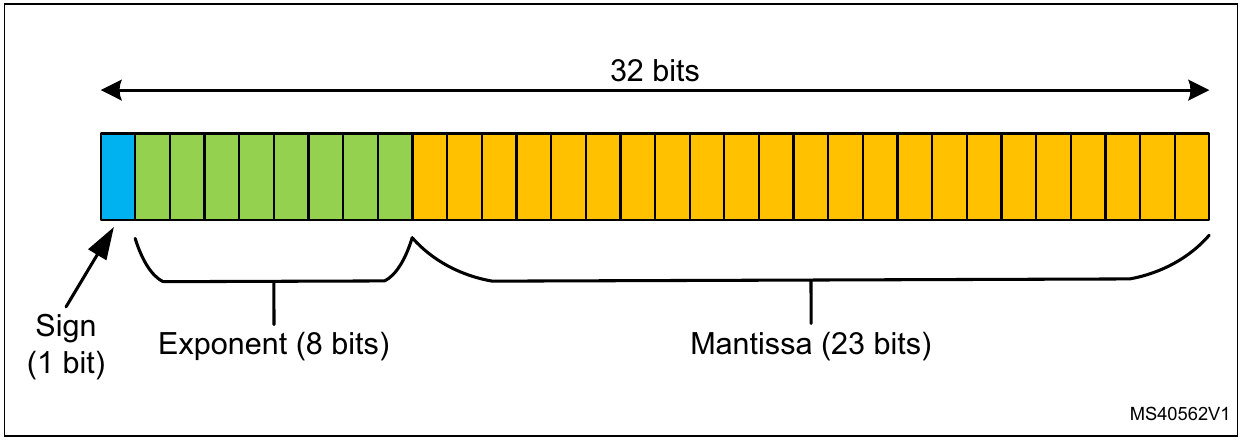
\includegraphics[width=\textwidth]{images/float}
    \caption{32-bit floating-point representation\cite{ST:DSP}.}
    \label{fig:Float}
\end{figure}

\section{Effects}
This section is dedicated to audio effects implemented in the devices
as well as their features and parameters.
It is important to fully understand nature of specific effect
in order to implement it's entire functionality in a proper way
\cite{Zolzer1},
\cite{Zolzer2},
\cite{Smith}.

\subsection{Delay}
Delay, also known as comb filter, is the most basic time based effect.
It creates echo of original signal,
which is delayed by specified amount of time.
This delayed signal is then mixed with original.
Delayed signal can also be attenuated and then fed back into a delay block
in order to achieve endless, fading reflections.

Figure \ref{fig:comb} presents block diagram of such a delay stage.
Z \(^{-M}\) block symbolizes a delay by M amount of samples.
Parameters FF (feedforward), FB (feedback) and BL (blend)
are representing gain of different signals.

\begin{figure}[H]
    \centering
    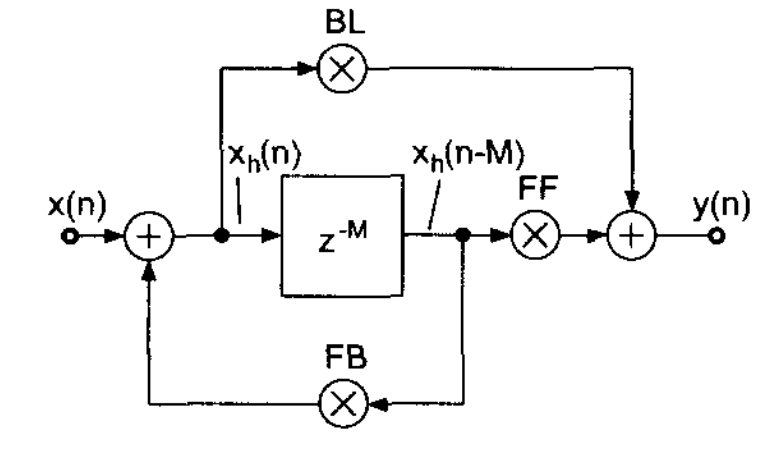
\includegraphics[width=0.618\textwidth]{images/comb}
    \caption{Universal comb filter\cite{Zolzer1}.}
    \label{fig:comb}
\end{figure}

Because processed signal is sampled,
delay time is described by number of samples.
Digital implementation of this effect requires use of circular buffer,
which size is determined by delay time required.
Each sample collected from input is stored in the buffer
in order to be read later and mixed to the output.

\subsection{Modulation}
Modulation effects use LFO (eng. Low frequency oscillator) to modulate different parameters.
Our attention will be focused on pitch modulation
which is based on delay effect and works by varying a delay time.
Modulation effects usually use short delay times up to 30ms
and LFO frequency up to several Hz.
Different functions, such as sine,
triangular or sawtooth can be used for LFO.

\begin{figure}[H]
    \centering
    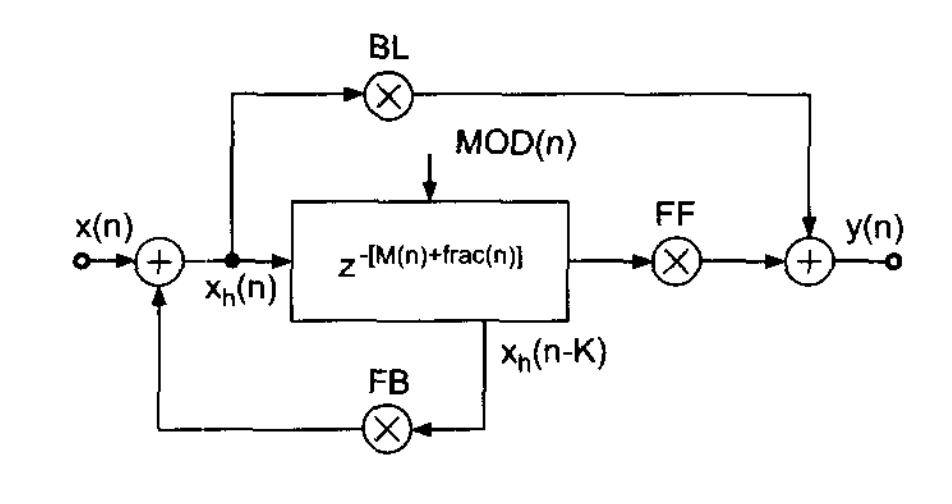
\includegraphics[width=0.7\textwidth]{images/modulation}
    \caption{Block diagram of standard effect with variable delay line\cite{Zolzer1}.}
    \label{fig:Mod}
\end{figure}

On the figure \ref{fig:Mod} we can see a block diagram of a
time-based modulation effect.
It is almost identical to diagram of comb filter,
only difference beeing a variable delay line.
Instead of delaying input signal by constant number of samples,
length of delay line changes in time
and is determined by a modulation function.

There are a few distinct modulation effects:
\begin{itemize}
    \item Chorus - uses delay time up to 20ms with LFO frequency up to 10Hz with medium depth.
    \item Flanger - simmilar to chorus, but uses shorter delay time and higher value of depth.
        Flanger effects also use feedback.
    \item Vibrato - is a different type of pitch modulation effect. It mutes original (dry) signal
        from the mix, leaving only modulated sound.
    \item Tremolo - in contrast to previous effects uses volume modulation instead of pitch modulation.
    \item Phaser - modulates phase of the signal. It is done with use of all-pass filters.
\end{itemize}

\subsection{Biquad filter}
Biquad (biquadratic) filter is a type of second order IIR digital filter.
The biquad filter is desctibed by 5 coefficients and exists in two direct forms.
Biquad filter is described by following transfer function:

\(H(z) = \frac{b_0 + b_1z^{-1} + b_2z^{-2}}{1 + a_1z^{-1} + a_2z^{-2}}\)

The difference between direct forms is that the direct form 1 uses four delay registers
while direct form 2 requires only two.
This is the reason why direct form 2 is more efficient and considered to be canonical.
Figure \ref{fig:biquad2} shows block diagrams of two different
direct forms of a biquad filter.

Use of proper formulas allows to implement biquad as one of many types of filters
including high-pass, low-pass, band-pass, peak, notch, high-shelf and low-shelf.
Filters are also described by parameters such as corner frequency, quality factor
and in some cases preak gain.
Figure \ref{fig:biquad} shows characteristics of some filters,
that can be implemented using biquad algorithm
\cite{Biquad},
\cite{biquad_web}.

\begin{figure}[H]
    \centering
    \begin{subfigure}[t]{0.55\textwidth}
        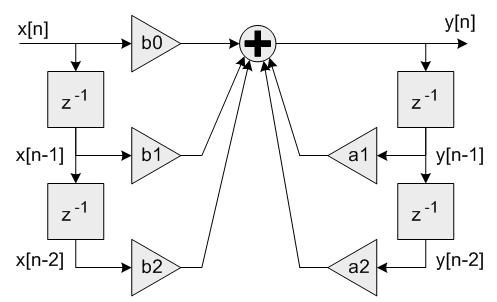
\includegraphics[width=\textwidth]{images/DF1}
        \label{fig:df1}
        \caption{Direct form I}
    \end{subfigure}
    ~
    \begin{subfigure}[t]{0.4\textwidth}
        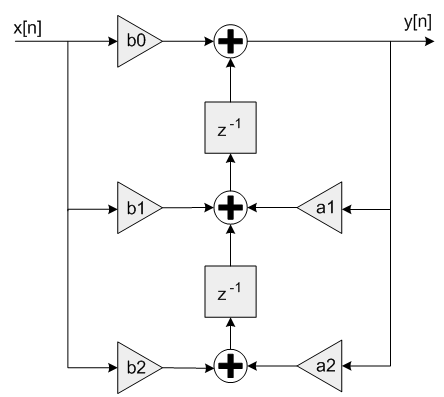
\includegraphics[width=\textwidth]{images/DF2}
        \label{fig:df2}
        \caption{Transposed direct form II}
    \end{subfigure}
    \caption{Direct forms of the biquad filter\cite{CMSIS_DSP}.}
    \label{fig:biquad2}
\end{figure}

\begin{figure}[H]
    \centering
    \begin{subfigure}[t]{0.8\textwidth}
        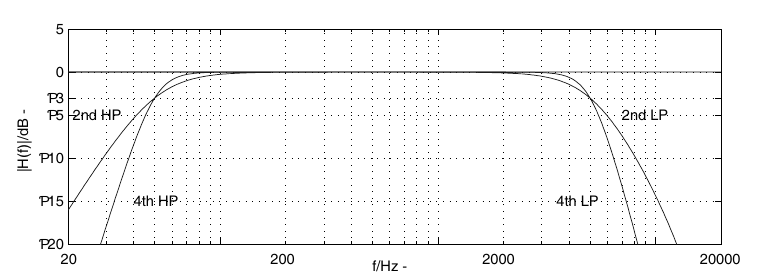
\includegraphics[width=\textwidth]{images/filter_pass}
        \label{fig:pass}
        \caption{High and low-pass filters}
    \end{subfigure}
    ~
    \begin{subfigure}[t]{0.4\textwidth}
        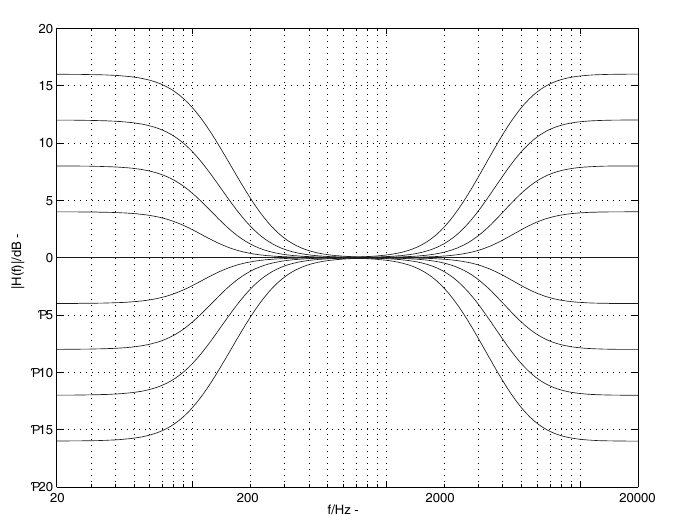
\includegraphics[width=\textwidth]{images/filter_shelving}
        \label{fig:shelf}
        \caption{Shelving filter}
    \end{subfigure}
    ~
    \begin{subfigure}[t]{0.4\textwidth}
        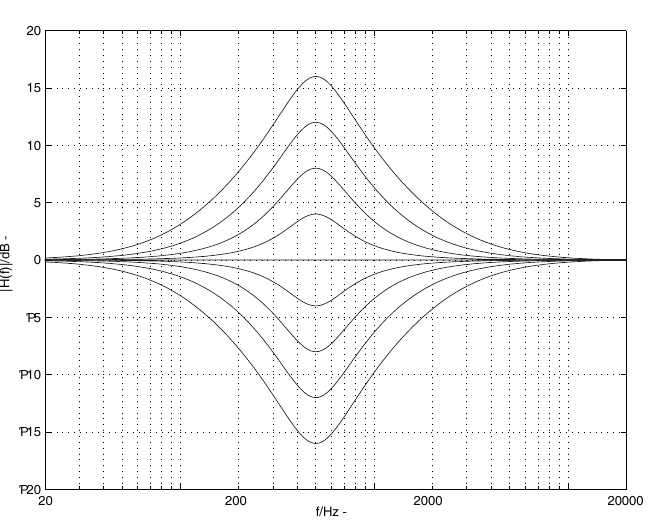
\includegraphics[width=\textwidth]{images/filter_peak}
        \label{fig:peak}
        \caption{Peak filter}
    \end{subfigure}
    \caption{Some kinds of filters, that can be implemented using biquad\cite{Zolzer2}.}
    \label{fig:biquad}
\end{figure}

\subsection{Drive}
Non-linear effects, such as overdrive, distortion or fuzz,
introduce higher harmonic frequencies into processed signal by clipping.
It is done by passing input signal through a non-linear clipping function.
This kind of effects are often used by guitarists,
especially these playing in rock and metal bands.


\chapter{External specification}\label{ch:external}
The Chapter \ref{ch:external} presents description of hardware components used in this project.

\section{Block diagram}
Figure \ref{fig:block} shows a block diagram of the device.
All external components are presented around a microcontroller
alongside with necessary connections.

\begin{figure}[H]
    \centering
    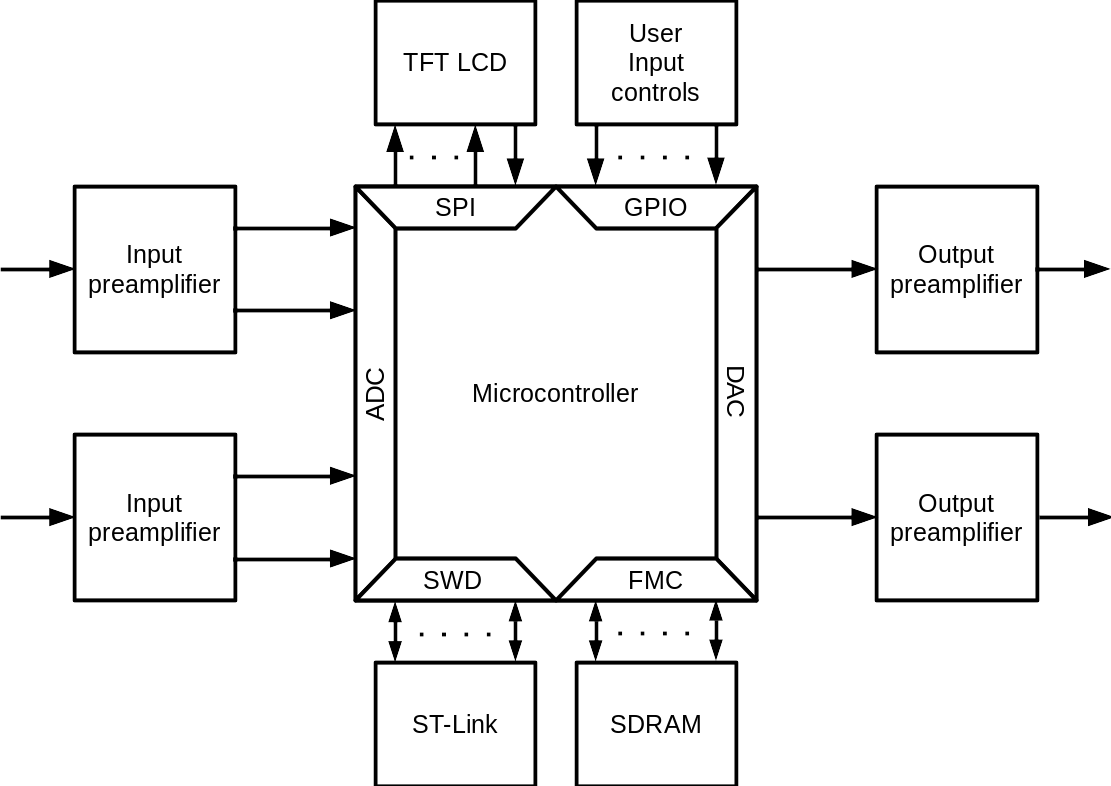
\includegraphics[width=0.75\textwidth]{images/Block}
    \caption{Block diagram of device.}
    \label{fig:block}
\end{figure}

\section{Construction of the device}
This section is devoted to choice of elements
and description of their arrangement.

\subsection {Microcontroller}
The microcontroller should meet certain parameters to be chosen.
One of the most important parameters is the clock speed.
Digital signal processing requires a lot of processor instructions
per each audio sample, so high clock speed is preferred.

The second important criterion is amount of memory.
The microcontroller should have at least 128kB of ROM
to fit the written program.
Size of RAM should be as high as possible,
because delay effects require a lot of memory.

Presence of FPU (eng. Floating-point unit) is preferred due to its performance benefits.
Dedicated floating-point hardware greatly decreases time
needed for floating-point calculations.

To reduce the total cost of the device,
proper A/D and D/A converters could be included in the microcontroller.

All of above criterion is met by STM32H743ZI microcontroller
\cite{ST:RM}.
It is based on Arm Cortex-M7 32-bit RISC core.
This specific model uses LQFP144 package.
Most important parameters of this microcontroller are listed below:
\begin{itemize}
    \item 480MHz maximum clock frequency
    \item 1MB of RAM and 2MB of Flash memory
    \item single and double precision FPU and set of DPS instructions
    \item 16-bit ADC and 12-bit DAC
    \item 140 I/Os and selection of peripherals such as hardware
    SPI, I2C, I2S, UART, SPDIF, USB OTG
\end{itemize}

\subsection{Development board}
The STM32H743ZI comes one the NUCLEO-H743ZI evaluation board,
which can be seen on figure \ref{fig:Nucleo}.

\begin{figure}[H]
    \centering
    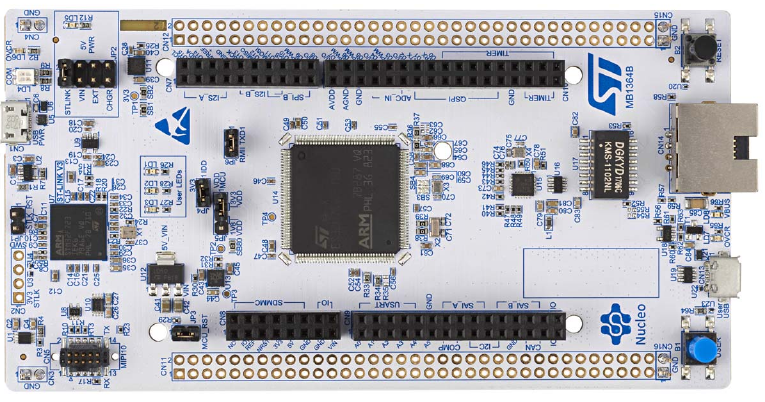
\includegraphics[width=\textwidth]{images/Nucleo}
    \caption{Nucleo H7 development board\cite{ST:UM2407}.}
    \label{fig:Nucleo}
\end{figure}

Device was designed in a form of a “shield” for Nucleo board.
The Nucleo board provides a ST-Link programmer/debugger
and voltage regulators required to power the board from 5V USB.
Clock signal can be acquired either from ST-Link or
external crystal oscillators.
Board also provides ethernet and USB OTG connectors,
which are not used in this project.

\subsection {Operational amplifiers}
TLC272C was operational amplifier of choice\cite{TI:TLC272}.
It contains two precision amplifiers in a single SOIC-8 package.

Analog power supply on the board is 3.3V, so the operational amplifier
must be capable of operating in such condition.
TLC272C is designed to work with single-supply configuration
and voltages as low as 3V,
while providing 2V of undistorted output voltage swing.

With normal operating conditions and at unity gain,
TLC272C has slew rate of 3.6 \(\frac{V}{\mu s}\) and bandwith of 1.7MHz.
Both of these parameters have values suitable for audio applications.

\subsection{Converters}
Device relays on both onboard digital to analog
and analog to digital converters present in the microcontroller,
so external preamplifiers are the only thing needed on the audio path.

\begin{figure}[H]
    \centering
    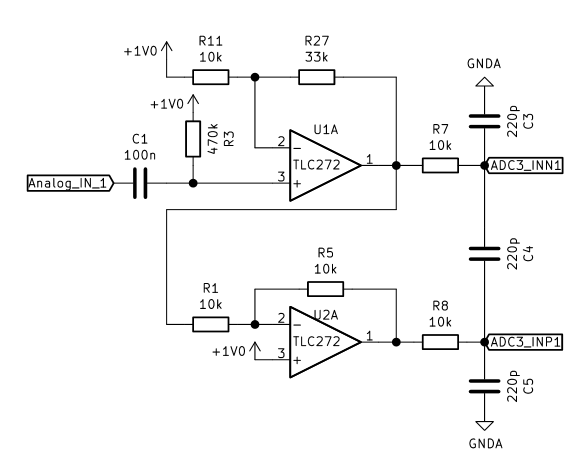
\includegraphics[width=0.75\textwidth]{images/Input_preamp}
    \caption{Schematic of input preamplifier.}
    \label{fig:input}
\end{figure}

Input preamplifier is preceded by a high-pass filter.
Purpose of this filter is DC isolation between sound source and preamplifier.
Cutoff frequency of this filter must be below 20Hz
in order to avoid losing meaningful data from the signal,
to keep some margin 3Hz was chosen.
Formula \ref{eq:RC} was used to determine values of C1 and R3.
Closest matching values of passive elements were chosen from E24 series.

\begin{equation}\label{eq:RC}
f_c = \frac{1}{2 \pi RC}
\end{equation}

Input preamp is designed to be a single-ended to differential converter.
First amplifying stage acts as a buffer and has gain equal to \(3\frac{V}{V}\).
Boost is added to improve performance of converters,
since line signal level is usually not higher than 900mVpp,
while reference voltage of ADC is equal to 3.3V.
This stage is designed as a non-inverting configuration of an operational amplifier.
Values of resistors were chosen using formula \ref{eq:noninverting}.

\begin{equation}\label{eq:noninverting}
k = 1+\frac{R_2}{R_1}
\end{equation}

At this point 1V DC offset is added, because unipolar voltage supply was used
and signal must be in the middle of our undistorted voltage range..
The second stage is a basic phase inverter with unity gain.
Resistors were selected using this formula \ref{eq:inverting}.

\begin{equation}\label{eq:inverting}
k = -\frac{R_2}{R_1}
\end{equation}

Outputs of both stages are fed into differential inputs of ADC
and are sampled by microcontroller.
To prevent aliasing and noise,
low-pass filter with both common-mode and differential-mode capacitors
is introduced. This filter is designed to provide 20kHz cutoff frequency.
values of pasive components were determined using formula \ref{eq:differenfial}
and selected from E24 series
\cite{aliasing}.

\begin{equation}\label{eq:differenfial}
f_{DM} = \frac{1}{2 \pi (R_7 + R_8)(C_4 + \frac{C_3 or C_5}{2})};\ for \ C_3 = C_5
\end{equation}

\begin{figure}[H]
    \centering
    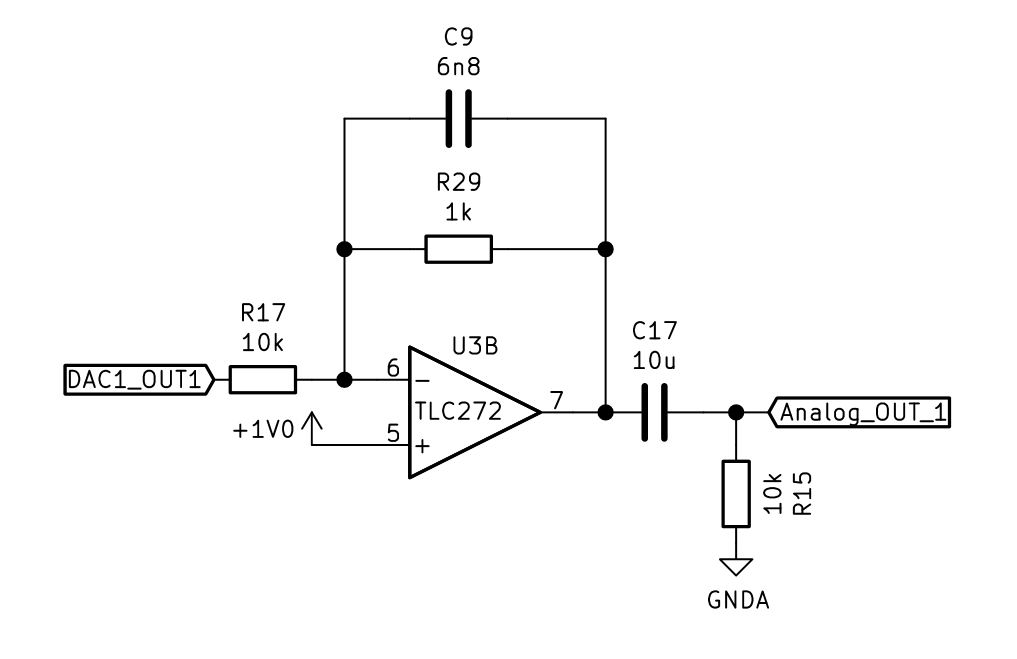
\includegraphics[width=0.75\textwidth]{images/Output_preamp}
    \caption{Schematic of output preamplifier.}
    \label{fig:output}
\end{figure}

Output preamplifier consist of single inverting operational amplifier.
This part of the circuit is based on suggestions from 
an application note \cite{ST:DAC}.
Output stage provides \(0.1\frac{V}{V}\) gain necessary to prevent
signal from clipping in potential receiving device.
After output stage there is a 1.5Hz high-pass filter,
whose task is to eliminate DC offset.
Values of C17 and R15 were calculated using formula \ref{eq:RC}.

\subsection{Display}
TFT LCD is required to provide necessary information to the user.
There are different ways to connect LCD to a microcontroller.
The most common is use of a parallel interface,
such as Intel 8080, Motorola 6800 or RGB interface.
These solutions require 8, 16 or 24 data lines,
alongside few other control signals.
Other approach involves use of serial interface,
such as SPI or I\(^2\)C.
It allows to reduce number of connections necessary to control the display,
at cost of greatly decreased data transfer rate.

With connection between MCU and LCD established,
we can focus our attention on actually sending data to be displayed.
Common approach, seen in TV and computer monitors,
is to constantly refresh the screen pixel by pixel.
It involves sending huge amounts of data,
even if displayed picture does not change.
Since most of LCD units designed to be used with microcontrollers
contain their own controller as well as RAM,
constant refreshing is completely unnecessary.
Instead, controller allows selecting a rectangular portion
of screen, which is ment to be updated.
This way we can eliminate problem of wasting MCU performance
on resending the same data over and over.

This project does not require high resolution,
because only basic information must be provided for a user.
That is why ST7735 TFT LCD was selected.
It is 128x160 pixels dot matrix display
and has 1.8 inch diagonal.

Some vendors provide drivers for their displays.
Unfortunately they are usually implemented for Arduino
and use so called polling mode,
which blocks MCU for the time of data transfer.
It means that custom driver must be created for this project.

\subsection{User interraction}
To allow user to interact with the device, a rotary encoder was introduced.
It is connected to microcontroller and is handled by internal timer.
By rotating the knob, user can navigate in the menu
in order to modify parameters and change an active effect.
Push button of the encoder and additional user button are connected
to GPIOs of the microcontroller with external pull-up resistors.
Buttons allow user to select different modes in menu.
User interface navigation is explained in details
in section \ref{ch:manual}.

\subsection{Additional devices}
Additionally the board is equipped with 32MB SDRAM chip
(of which only 16MB is accessible).
It is not used by the program of this project, but allows for future improvements.
SDRAM is handled by FMC (eng. Flexible memory controller) present in the microcontroller.

\section{Schematic}
Schematic was created using KiCad EDA,
which is both cross-platform and open source software.
It provides rich library of components and very intuitive user interface.

Schematic is divided into three parts,
each containing components related to each other.
Analog part, presented on figure \ref{fig:Schematic1}, is devoted to input and output amplifiers.
In digital section, on figure \ref{fig:Schematic2}, we can find external memory, LCD and rotary encoder.
Figure \ref{fig:Schematic3} presents the last part,
which is dedicated to gold pins connecting shield to a Nucleo board.

Power supply for a shield is provided by Nucleo board.
Digital and analog power sections are separated to reduce noise.
Use of local bypass capacitors was necessary to provide stable
supply voltage fo all different components in the circuit.

\begin{figure}[H]
    \centering
    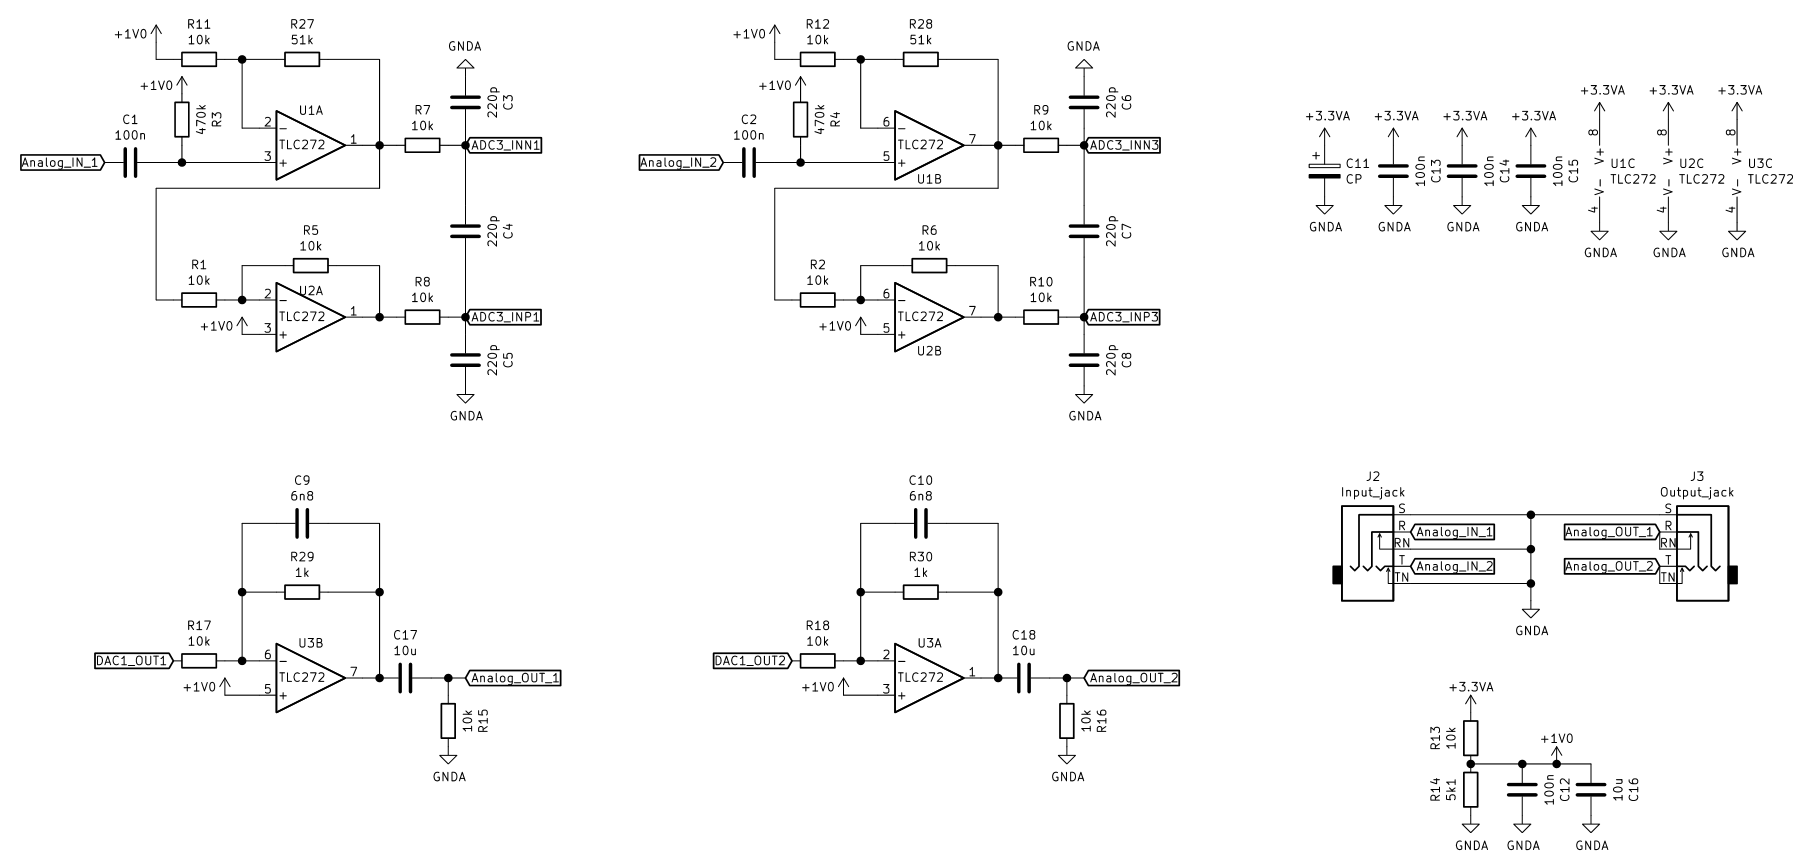
\includegraphics[width=\textwidth]{images/Schematic_analog}
    \caption{Schamatic of analog part of the device.}
    \label{fig:Schematic1}
\end{figure}

\begin{figure}[H]
    \centering
    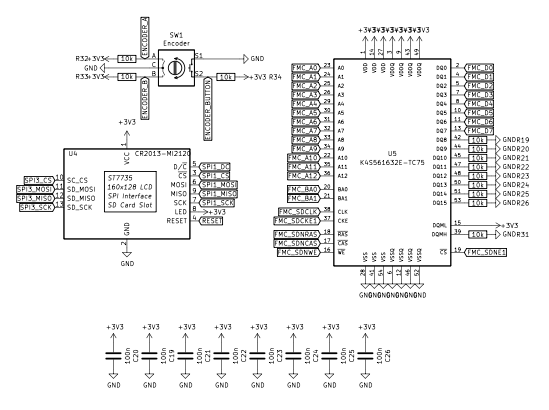
\includegraphics[width=0.8\textwidth]{images/Schematic_digital}
    \caption{Schamatic of digital part of the device.}
    \label{fig:Schematic2}
\end{figure}

\begin{figure}[H]
    \centering
    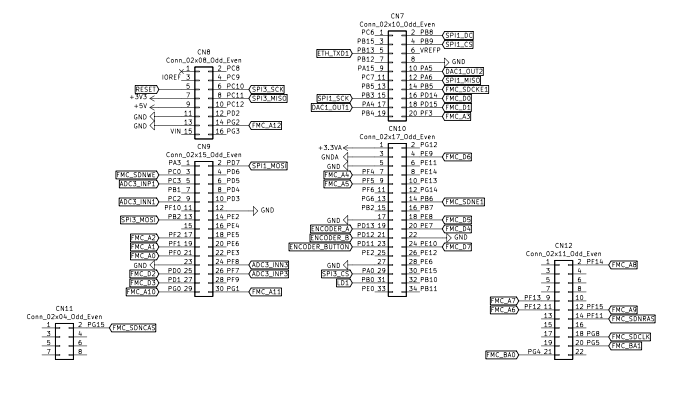
\includegraphics[width=\textwidth]{images/Schematic_connectors}
    \caption{Schamatic of gold pin connectors.}
    \label{fig:Schematic3}
\end{figure}

\section{PCB}
PCB layout was prepared using KiCad EDA as well.
All elements except for gold pin headers,
rotary encoder and audio jacks are SMD (surface mounted).
To reduce cost of the project, the PCB was designed as 2 layer board only.
This decision resulted in increased difficulty of routing process.

Since both analog and digital signals are present in the circuits
some extra steps were required during PCB design.
Important part was separation of grounds,
which resulted in two separate ground planes.
On figure \ref{fig:board} we can see copper and 
silkscreen layers of designed board.

\begin{figure}[H]
    \centering
    \begin{subfigure}[h]{0.273\textwidth}
        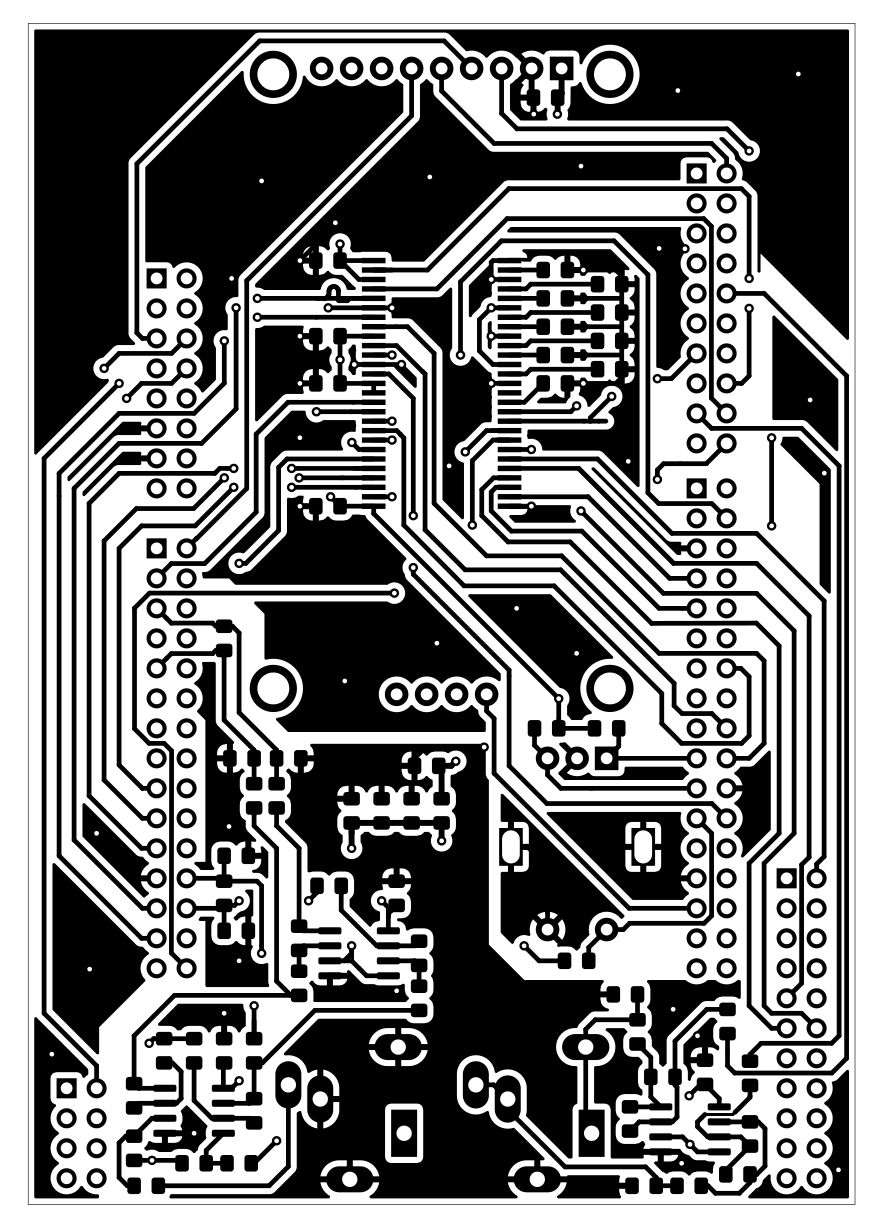
\includegraphics[width=\textwidth]{images/Board_front}
        \label{fig:board1}
        \caption{Front copper}
    \end{subfigure}
    ~
    \begin{subfigure}[h]{0.273\textwidth}
        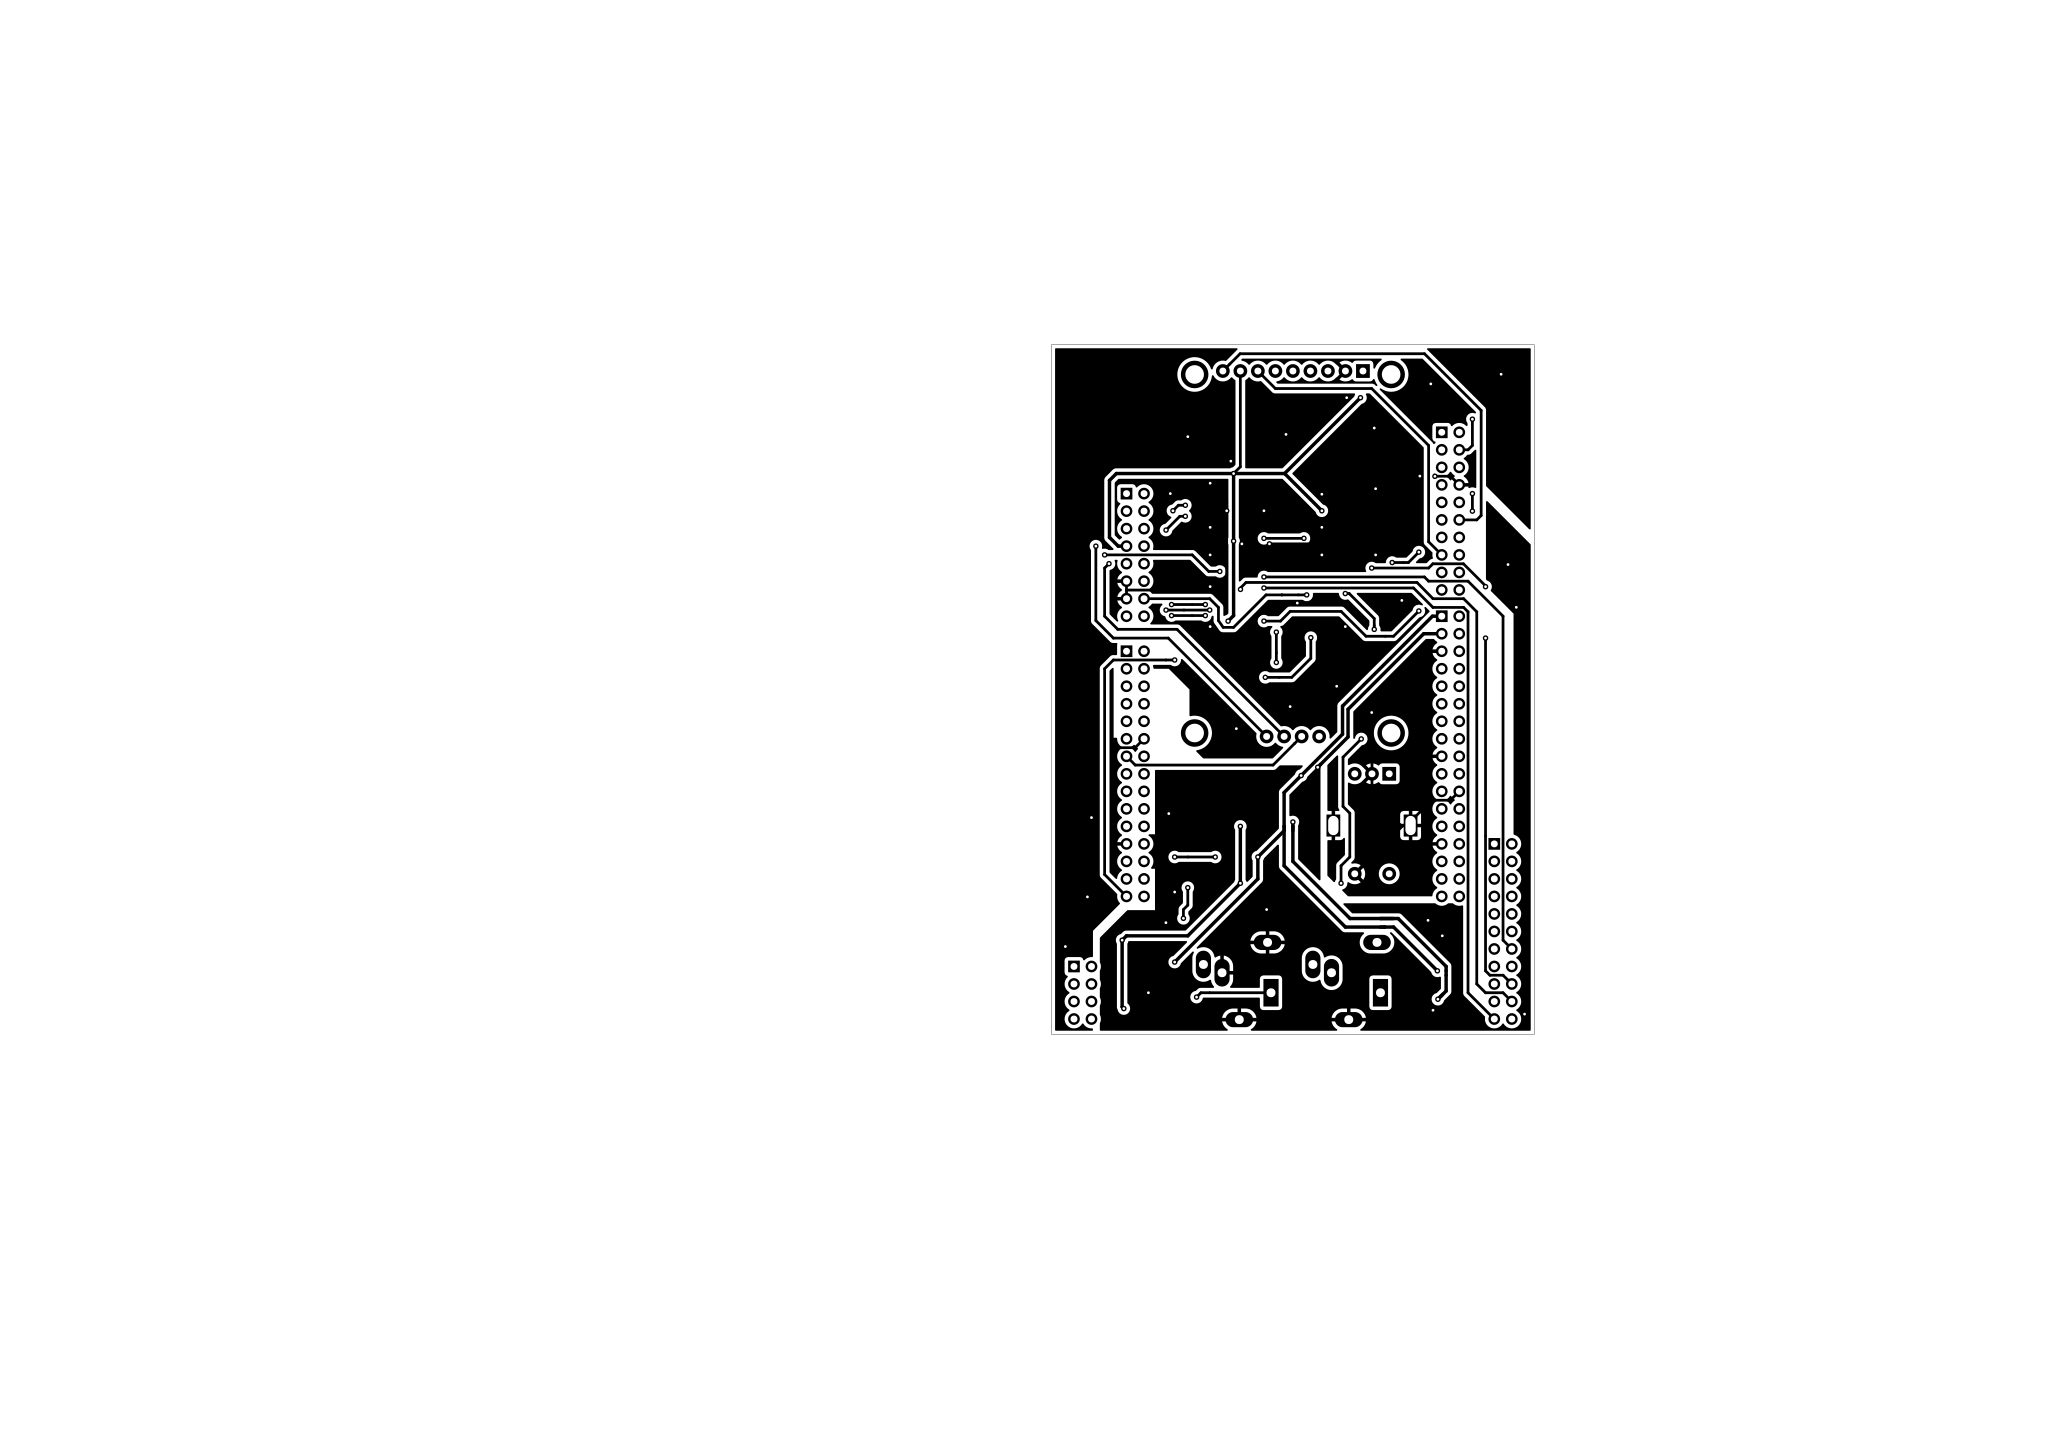
\includegraphics[width=\textwidth]{images/Board_back}
        \label{fig:board2}
        \caption{Back copper}
    \end{subfigure}
    ~
    \begin{subfigure}[h]{0.273\textwidth}
        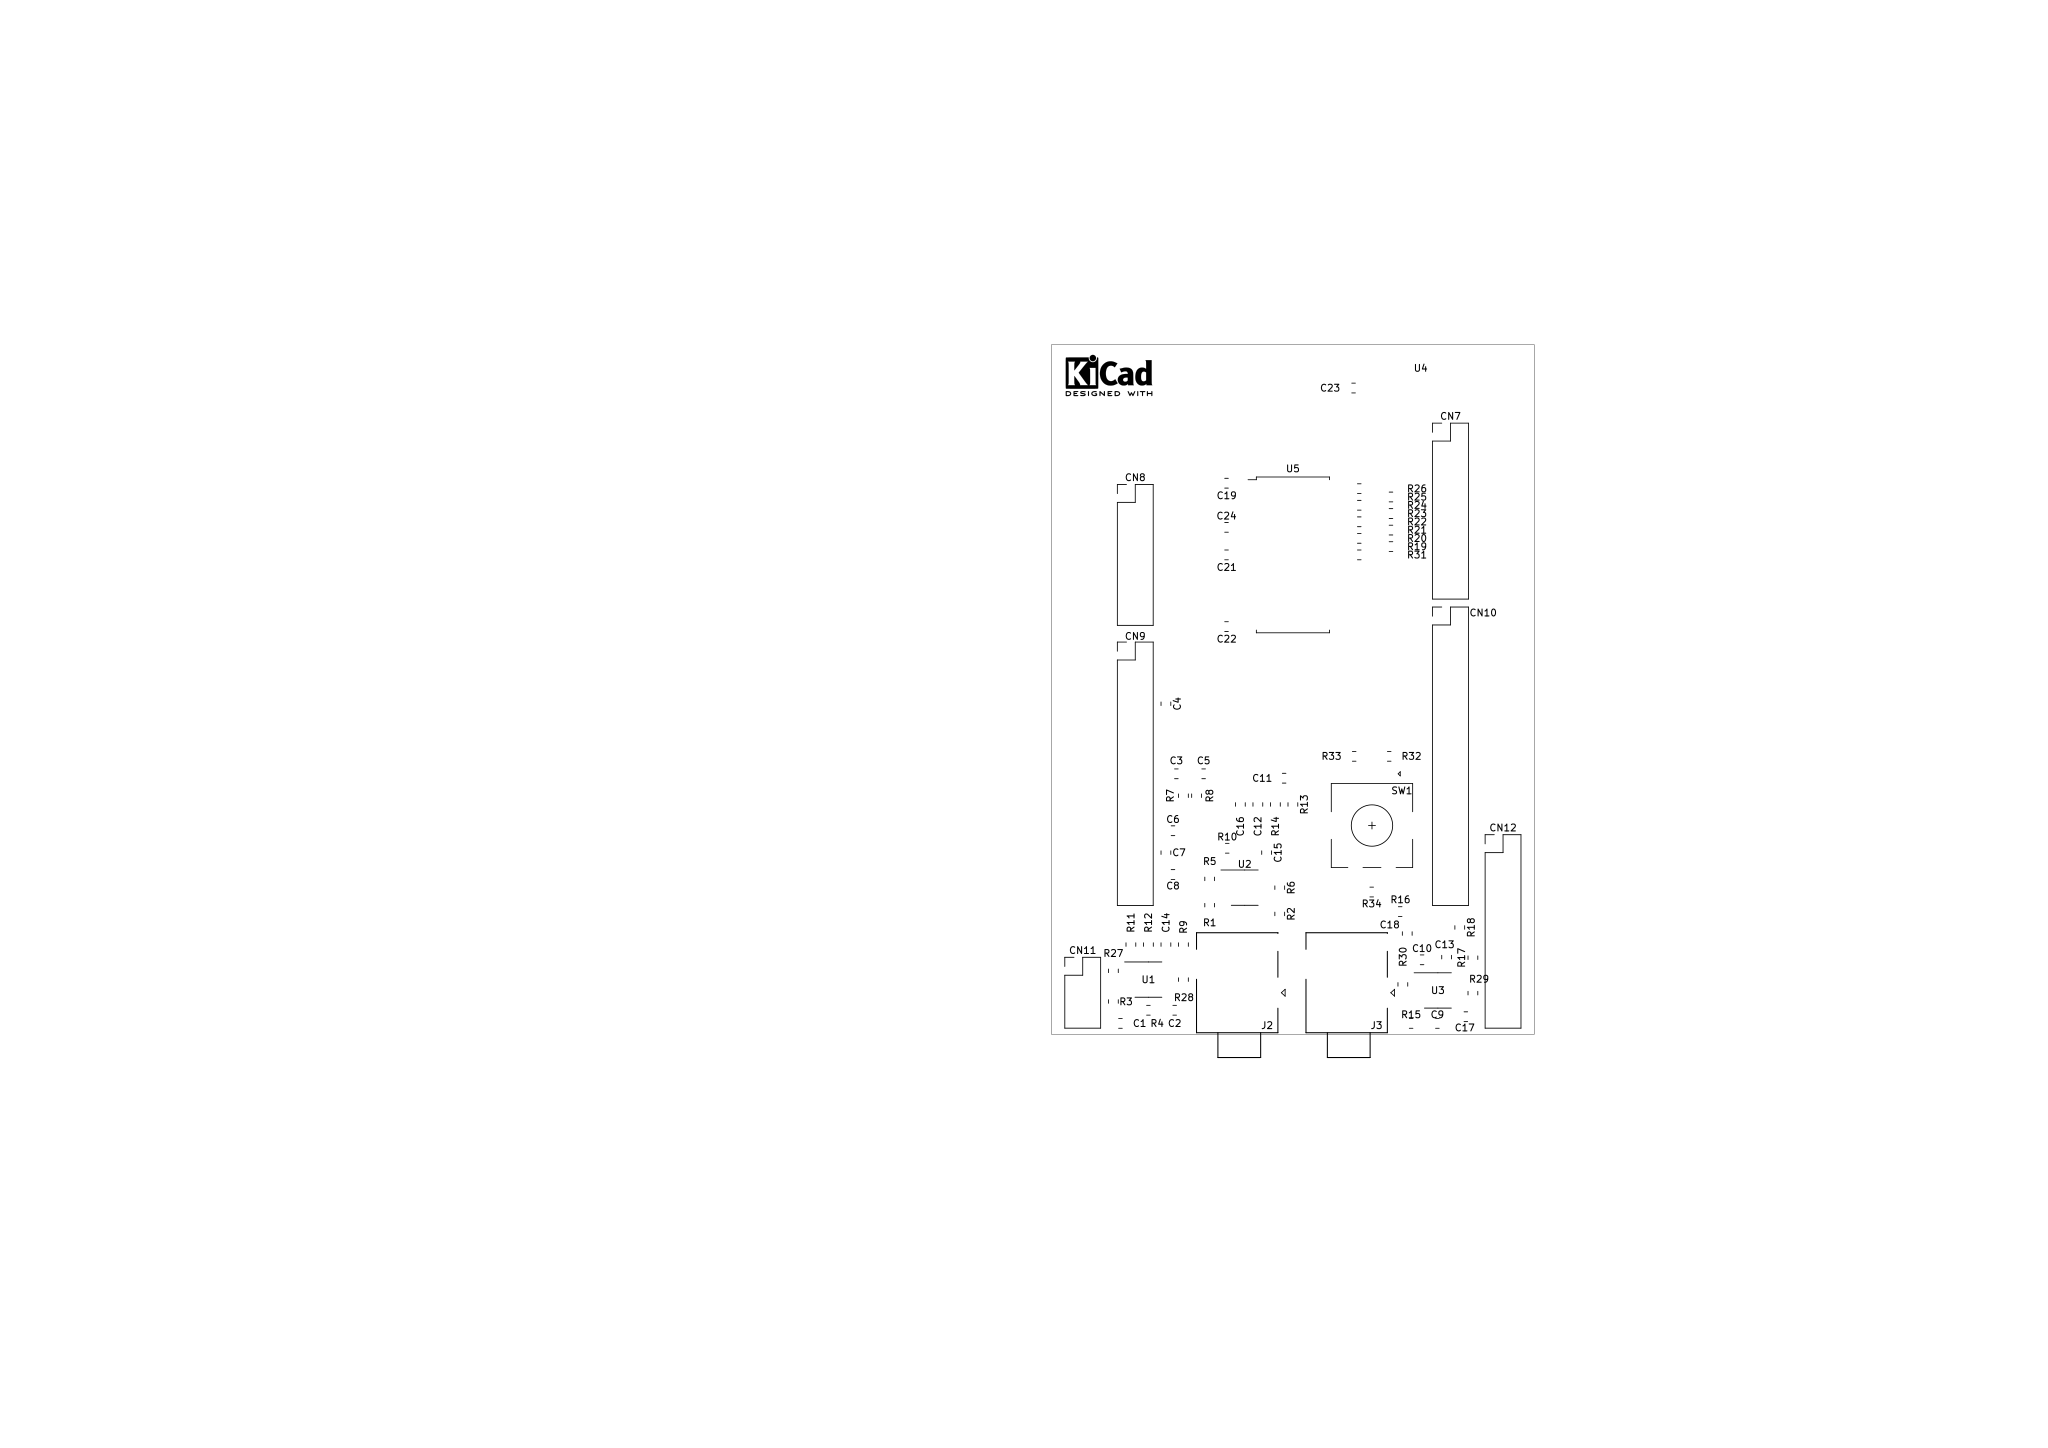
\includegraphics[width=\textwidth]{images/Board_silkscreen}
        \label{fig:board3}
        \caption{Front silkscreen}
    \end{subfigure}
    \caption{Copper and silkscreen layers of the PCB (1:2 scale).}
    \label{fig:board}
\end{figure}

Gerber files generated by the software were sent to manufacturer in China
and arrived two weeks later.
Manufectured boards can be seen on figure \ref{fig:photo_boards}.

\begin{figure}[H]
    \centering
    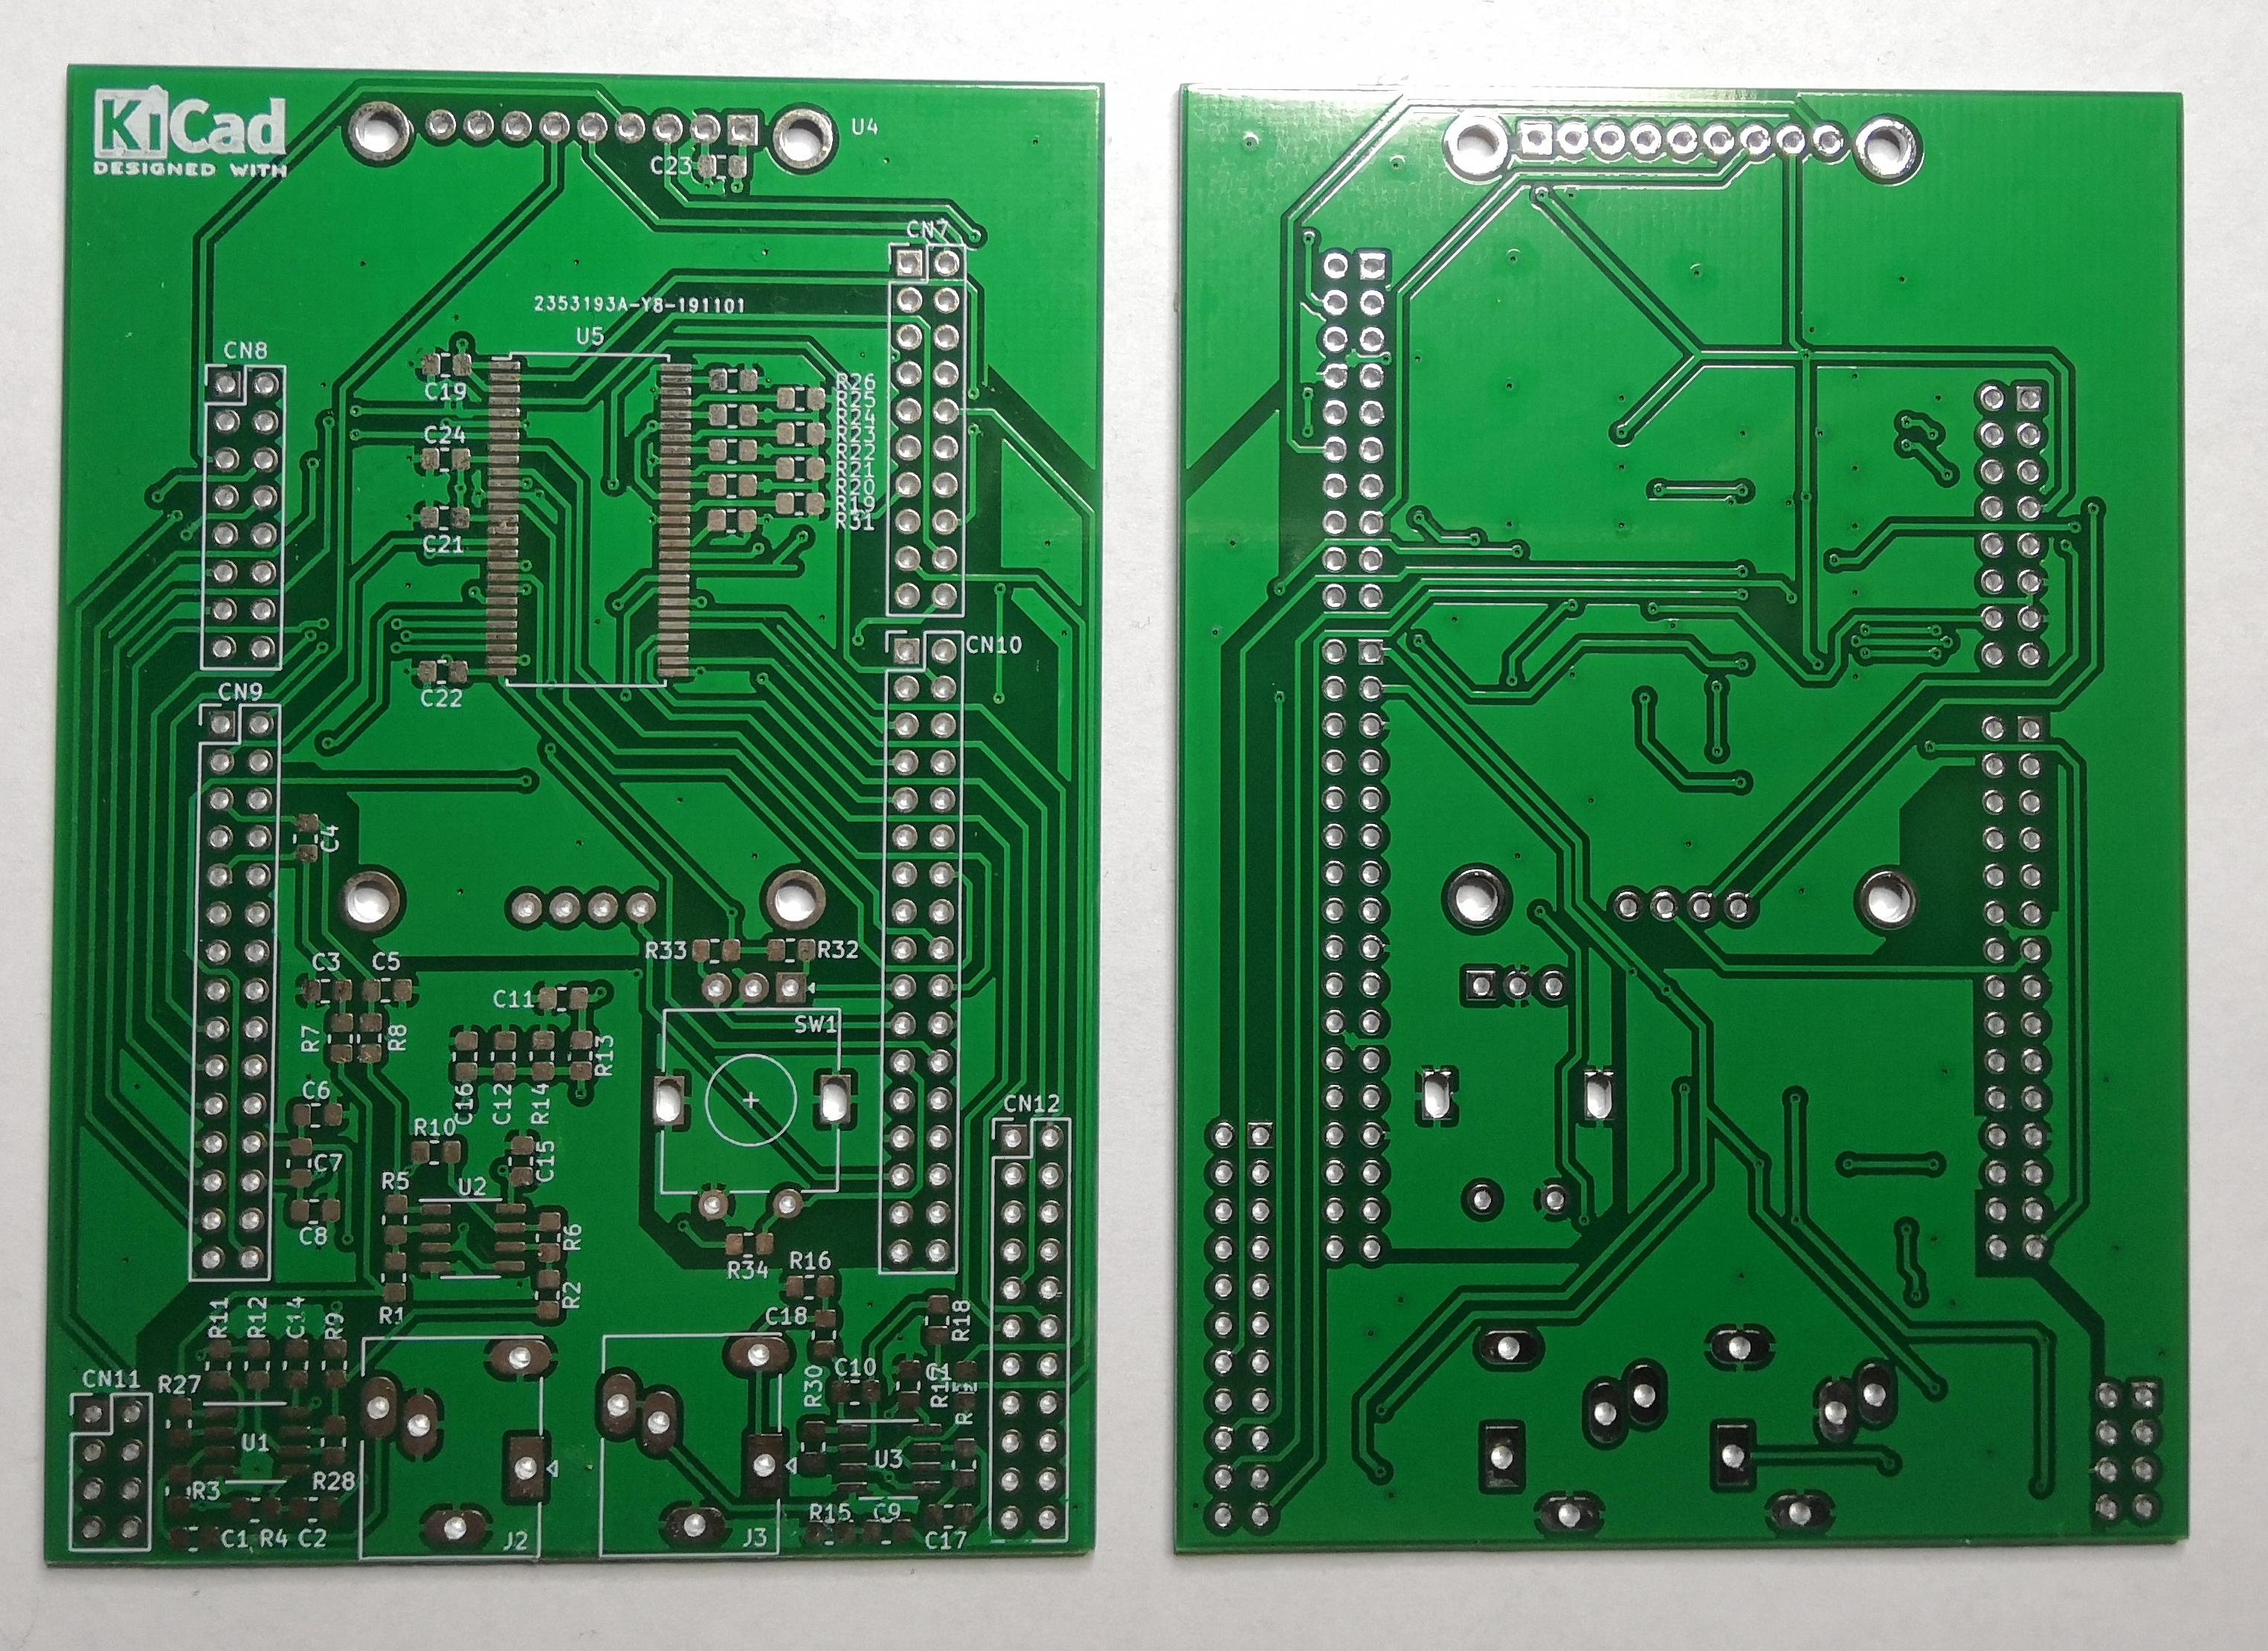
\includegraphics[width=0.618\textwidth]{images/photo_boards}
    \caption{Photo of front and back sides of the PCB.}
    \label{fig:photo_boards}
\end{figure}

\section{Assembly}
The PCB was populated by hand using 50W soldering iron and hot air rework station.
Two types of tin-lead solder were used during the process:
0.25mm solder wire (Sn60 Pb40) for THT components and solder paste (Sn62 Pb36 Ag2) for SMD.
Visualisation and photo of assembled board can be seen
on figures \ref{fig:pcb3d} and \ref{fig:photo_assembled}.

\begin{figure}[H]
    \centering
    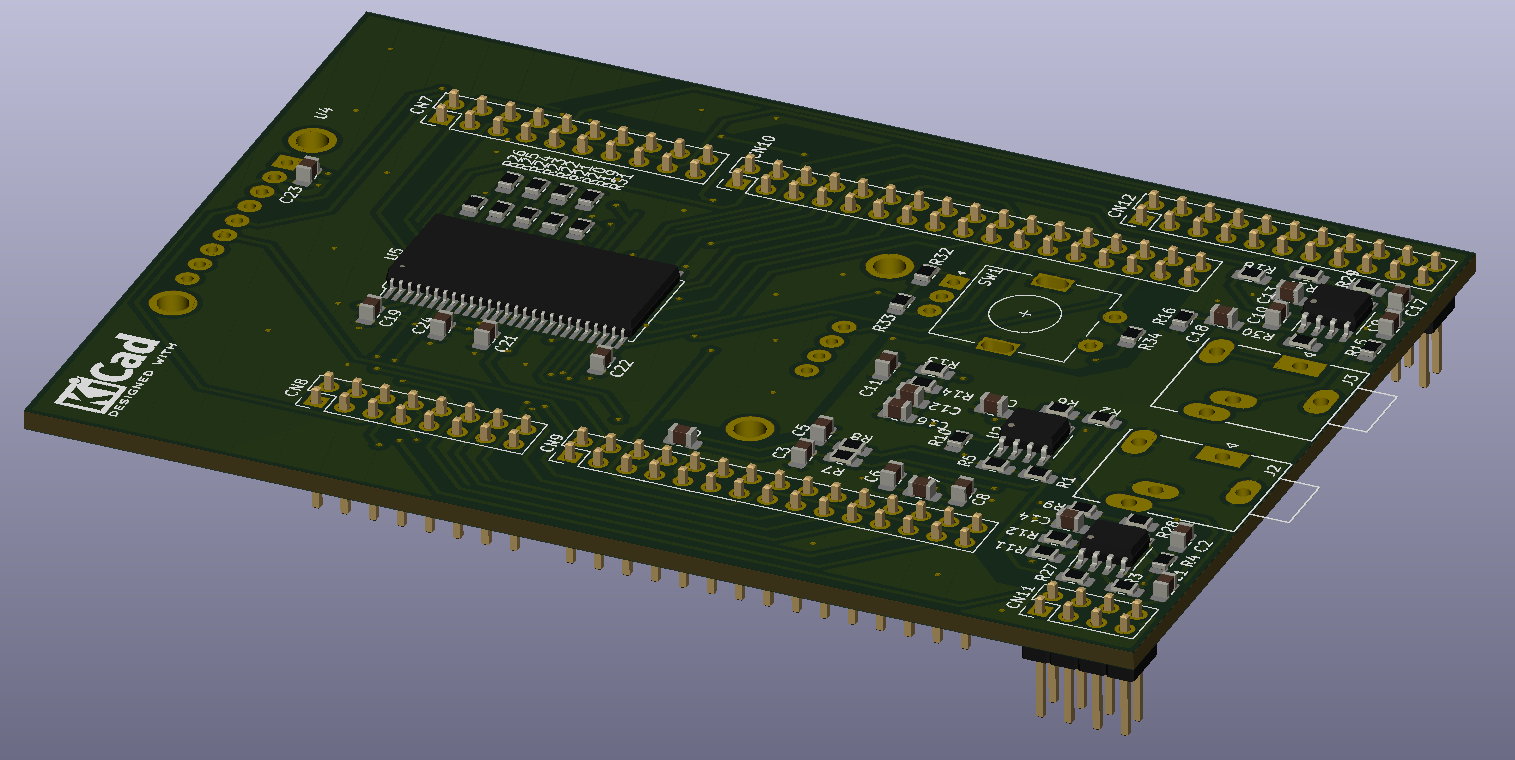
\includegraphics[width=0.9\textwidth]{images/PCB3D}
    \caption{3D render of the PCB.}
    \label{fig:pcb3d}
\end{figure}

\begin{figure}[H]
    \centering
    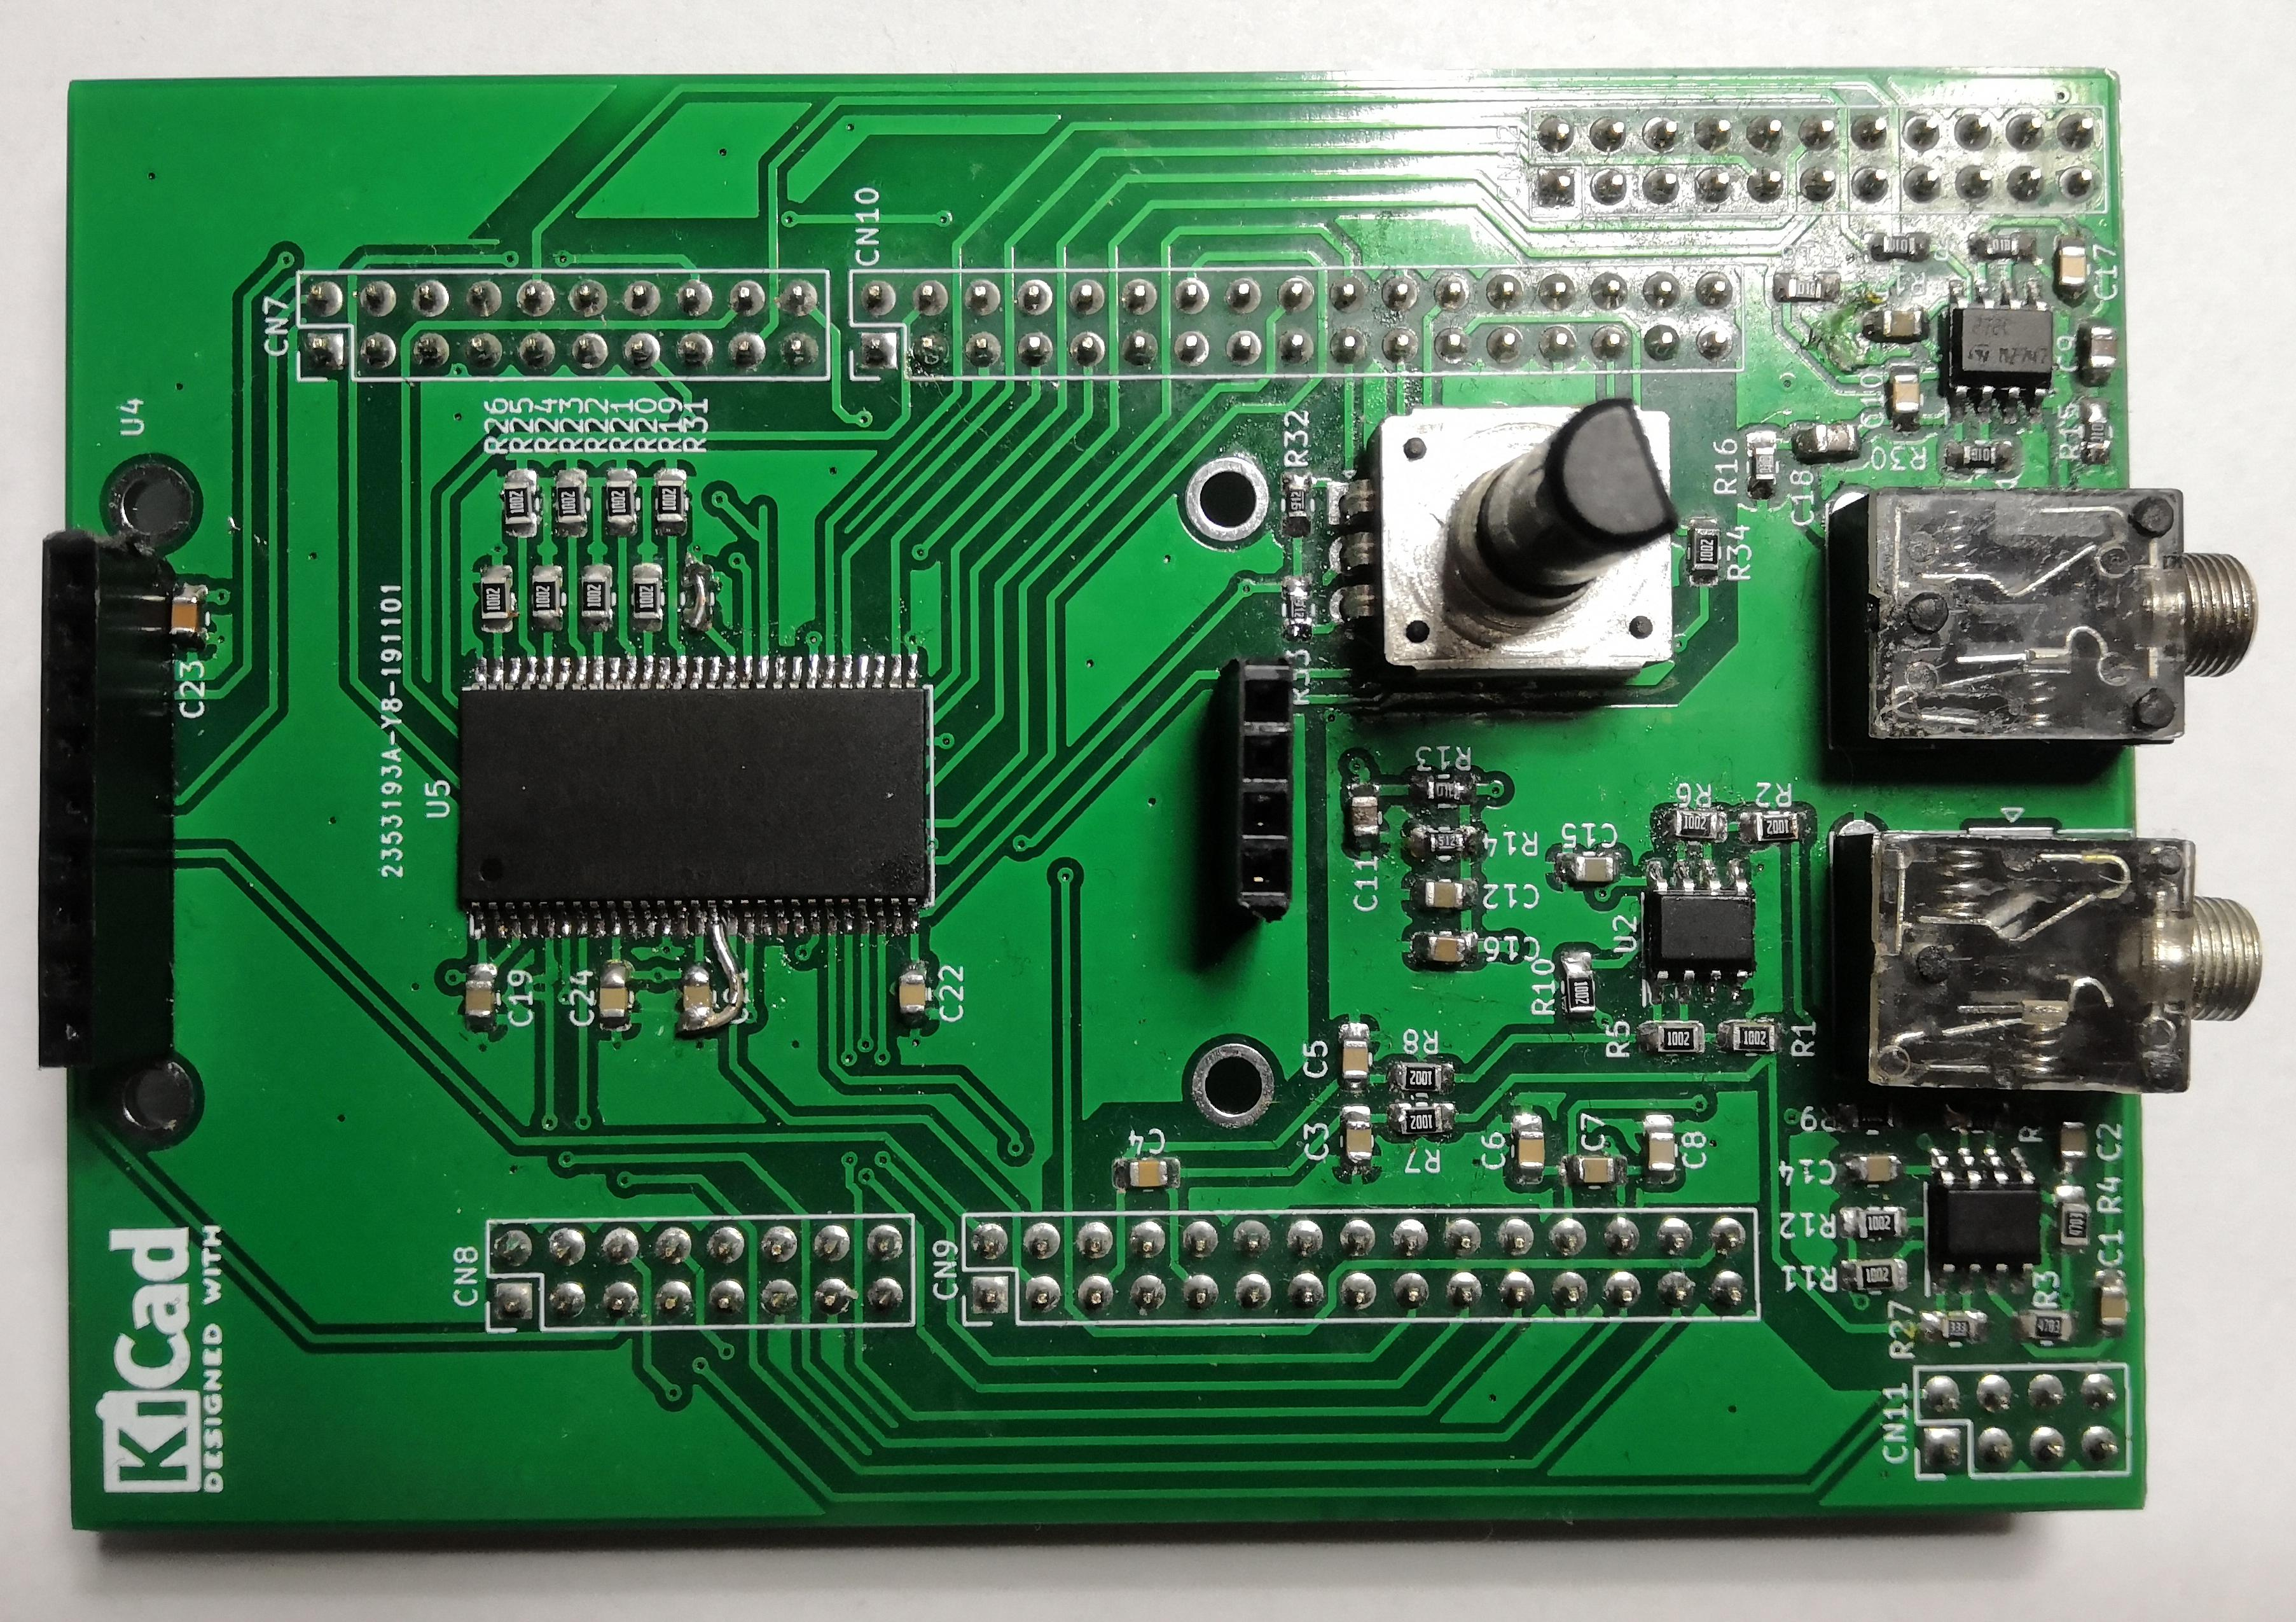
\includegraphics[width=0.618\textwidth]{images/photo_assembled}
    \caption{Photo of assembled board.}
    \label{fig:photo_assembled}
\end{figure}



\chapter{Internal specification}\label{ch:internal}
The chapter \ref{ch:internal} is devoted to choice of
programming tools and writing the program itself.

\section{Programming environment}
Programming environment consist of several tools,
that need to work together to facilitate software development.
All tools used in this project are free and cross-platform.
Following section is devoted to choice of these tools.

\subsection{Programming language}

C language is the most popular choice for STM32 development.
It is widely supported by ST and other companies providing frameworks and libraries.
As a low level language, it provides control over memory management,
which is a important factor in software development for microcontrollers.

Since the object oriented approach was preferred in this project,
C++ language was chosen.
This allows to benefit from libraries written in C,
but also gives advantages of using classes with inheritance and polymorphism,
which are part of C++ language.

\subsection{IDE}

The popular environments for STM32 development are Keil uVision and IAR.
ST also provides its own STM32CubeIDE, which is based on Eclipse.

Another choice is PlatformIO IDE.
It provides all libraries, frameworks,
debugger server and compiler necessary for STM32 software development.
It is free and open source IDE and
comes as a plugin for Visual Studio Code.

Visual Studio Code is a free code editor developed by Microsoft.
VSCode provides linting and word completion extensions,
which simplify the process of software development.

Combination of VSCode and PlatformioIDE was a very apealing option,
since it provides a modern user interface alongside with all necessary tools.
It was chosen as programming environment for both development and debugging
process of the projetc.

\subsection{Frameworks and tools}

List of frameworks and additional tools used for software development:

\begin{itemize}
    \item HAL drivers
    - Hardware Abstraction Layer driver is a library written in C language, provided by ST.
    It allows an easy use of microcontroller and code compatibility between different STM32 devices.
    \cite{ST:HAL}
    \item STM32CubeMX
    - a graphical tool that allows an easy STM32 configuration.
    It generates configuration code for the microcontroller and desired peripherals in C language.
    STM32CubeMX uses HAL driver in generated initialization code.
    \item CMSIS
    - Cortex Microcontroller Software Interface Standard
    is a hardware abstraction layer provided by Arm.
    It is compatible with all Arm Cortex microprocessors and microcontrollers.
    It includes API for Cortex-M and Cortex-A core and peripherals as well as additional tools
    (DSP library, neural network kernels, real-time operating systems).
    Especially DSP Library was useful during development of this project.
    \cite{CMSIS_DSP}
    \item OpenOCD
    - Open On-Chip Debugger provides programming and debugging support of boundary scan interface.
    It supports ST-Link, which was used for both programming and debugging of STM32 microcontroller.
    \item GNU Embedded Toolchain for Arm
    is a suite of tools for C, C++ and Assembly programming provided and maintained by Arm.
    It contains the GCC Compiler as well as linker.
    \item Git
    is a version control system. It allows to track changes in code
    and revert to any previous state.
    It can also act as a backup, because data can be stored on external server.
\end{itemize}

\section{Software block diagram}
On the figure \ref{fig:block2} we can see a software block diagram.
The diagram consist of two paths.
Part on the left shows a main path with all initialization procedures.
It also contains an infinite loop in which processor is waiting
for a block\_ready flag to be set.
This condition triggers action of processing a block of data.
During time between succesive data blocks,
processor updates the screen.

Second part is showing a timer interrupt.
It contains all instructions related
to reading from and writing to converters.
A block\_ready flag is set in this function
when input buffer is full of samples.

\newpage

\begin{figure}[H]
    \centering
    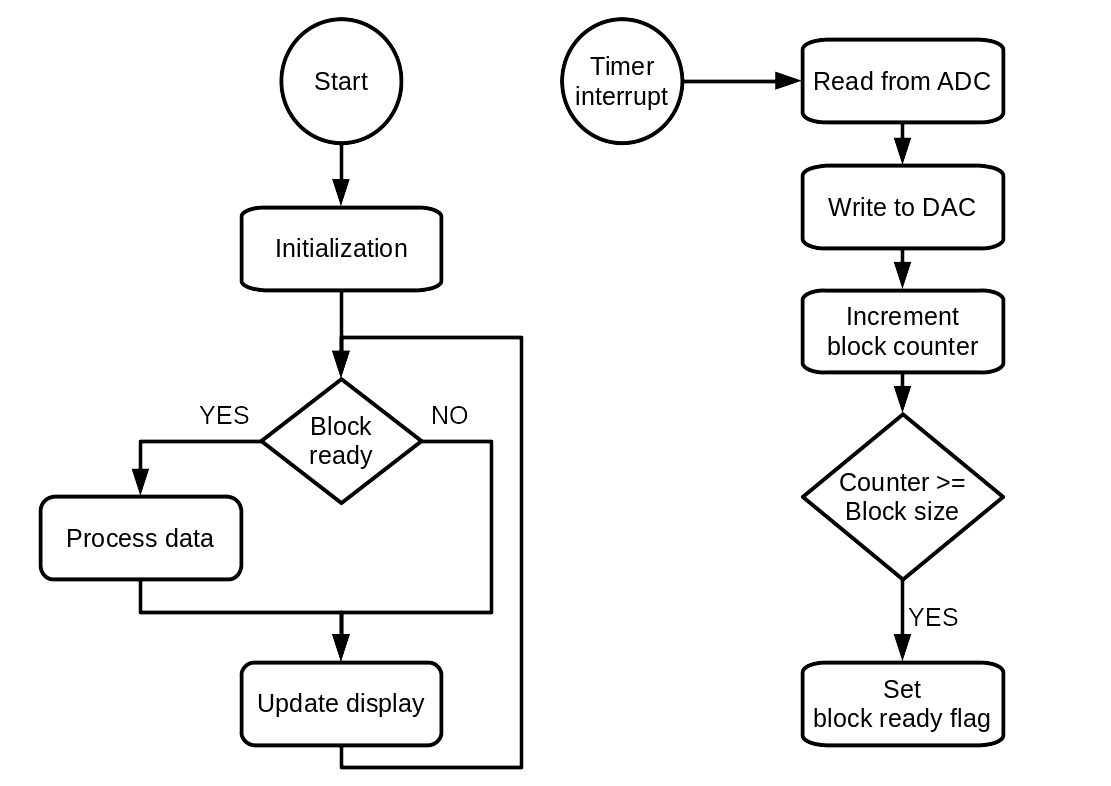
\includegraphics[width=\textwidth]{images/Block2}
    \caption{Block diagram of the program.}
    \label{fig:block2}
\end{figure}

\section{Configuration}
This section is dedicated to all configurations necessary to start programming.
It involves configuration of GPIO of a microcontroller as well as
many other peripheral devices.

\subsection{Code generation}

Initialization code was generated using STM32CubeMX software.
It provides necessery implementation of initialization functions
as well as general structure of the program.
Each enabled peripheral has its own source file
and corresponding header file.
Figure \ref{fig:pins} shows pin configuration of STM32H743ZI
generated using STM32CubeMX software.
Green pins are configured and used, yellow are pins reserved by
devices present on Nucleo board and grey are not used at all.

\begin{figure}[H]
    \centering
    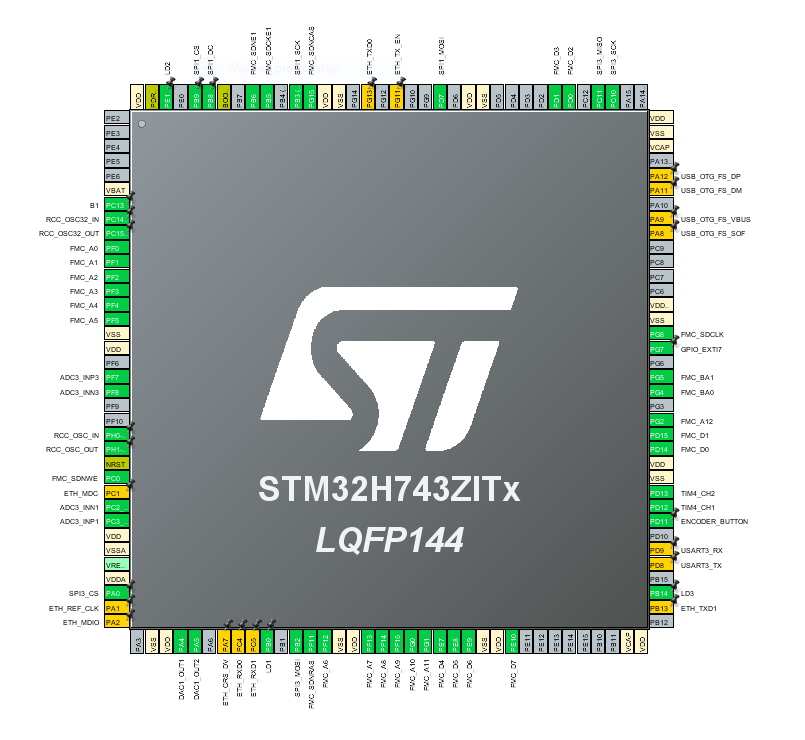
\includegraphics[width=\textwidth]{images/pin_overview}
    \caption{Screenshot of the pin configuration in STM32CubeMX software.}
    \label{fig:pins}
\end{figure}

\subsection{Clock}

Clock cource is set to be HSE (eng. High speed external),
it means that external crystal oscillator is used to
provide stable clock frequency.
Maximum clock frequency for this version of MCU is supposed to be 480MHz,
but microcontroller did not work properly with clock speed above 400MHz.
Unfortunately 400MHz is not divisible by 48kHz, which is our sampling frequency.
For that reason clock prescalers are set to obtain 396MHz clock frequency.
This way it is easy to setup desired sampling frequency on one of the timers.
This timer is used to generate interrupts with frequency of 48kHz,
which are necessacy for both ADC and DAC.
Clock was also configured using STM32CubeMX software.

\subsection{Environmental settings}

All settings passed to tools such as linter, compiler and linker
are present in platformio.ini and extra\_script.py files.
These settings give information about used frameworks
and paths to specific libraries and header files
\cite{platformio},
\cite{gcc}.

\begin{figure}[H]
\centering
\begin{lstlisting}
[platformio]
include_dir = ./Inc

[env:nucleo_h743zi]
platform = ststm32
board = nucleo_h743zi
framework = stm32cube
board_build.f_cpu = 396000000L
board_upload.maximum_ram_size = 65536
build_flags =   -I ${PROJECT_PACKAGES_DIR}/framework-stm32cube/h7/Drivers/CMSIS/DSP/Include
                -I ${PROJECT_PACKAGES_DIR}/framework-stm32cube/h7/Drivers/STM32H7xx_HAL_Driver/Inc
                -L ${PROJECT_PACKAGES_DIR}/framework-stm32cube/h7/Drivers/CMSIS/Lib/GCC
                -l libarm_cortexM7lfsp_math.a
                -D ARM_MATH_CM7
                -D __FPU_PRESENT=1
extra_scripts = pre:extra_script.py
\end{lstlisting}
\caption{Contents of platformio.ini file.}
\label{fig:ini}
\end{figure}

\subsection{FPU}

Floating-point unit present in the microcontroller must be enabled
using special compiler flags. Without them program would be compiled
using software floating-point, which is very slow and unefficient.
-mfpu=fpv5-d16 flag specifies version of Arm FPU present in microcontroller.
-mfloat-abi=hard forces to compile with hardware floating-point.
Both of them are set in extra\_script.py file.

\subsection{Cache}

STM32H7 series of microcontrollers provide both data and instruction cache.
This kind of memory can enhance performance of the device,
since it is twice as fast as other sections of RAM.
Despite the performance gain, cache (especially data cache)
must be used with caution, since it can cause some issues with DMA.
\cite{dma}
The solution involves using cache clear and invalidation functions.
These function forces transfer between RAM and cache in order to ensure,
that DMA is referencing valid data.

\subsection{Memory organization}
Memory in STM32H743 microcontrollers is divided into several segments,
which can be seen on figure \ref{fig:mem}.

\begin{figure}[H]
\centering
\begin{lstlisting}
ITCMRAM (xrw)   : ORIGIN = 0x00000000, LENGTH = 64K
FLASH (rx)      : ORIGIN = 0x08000000, LENGTH = 2048K
DTCMRAM (xrw)   : ORIGIN = 0x20000000, LENGTH = 128K
RAM_D1 (xrw)    : ORIGIN = 0x24000000, LENGTH = 512K
RAM_D2 (xrw)    : ORIGIN = 0x30000000, LENGTH = 288K
RAM_D3 (xrw)    : ORIGIN = 0x38000000, LENGTH = 64K
SDRAM (xrw)     : ORIGIN = 0xD0000000, LENGTH = 16M
\end{lstlisting}
\caption{Memory areas specified in linker script.}
\label{fig:mem}
\end{figure}

2MB of FLASH is used to store a program instructions and non-volatile data.
ITCMRAM and DTCMRAM regions are cache memory.
Main RAM memory was chosen to be located at RAM\_D3 region.
It is only 64k, but it is big enough to allocate all object and variables.
RAM\_D2 is reserved exclusively for DMA buffers,
which must be properly aligned in memory.
Last used memory region is 512kB RAM\_D1.
In this section all delay buffers are placed.
They are located there, because they take a lot of space.

\subsection{Timer}
There are two timers used in this project.
TIM4 is used to handle rotation encoder.
It counts impulses to determine number of turns 
performed by the user.
Second timer, used to determine sampling frequency, is TIM2.
It is set up to generate an interrupt every 20.8us,
which corresponds to 48kHz sampling frequency.

\subsection{ADC}
ADC is set to continuous conversion mode.
It is constatnly converting signal with sampling rate above 100kHz.
Obtained samples are then transfered to a buffer using DMA.
Parallel to ADC, a timer is generating interrupts
with rate equal 48kHz. During such interrupt,
freshest sample is copied into block buffers. 
When the block buffer is full, it can be swaped with empty buffer
and than processed.

\subsection{DAC}
DAC implementation was much easier than ADC.
Output samples are passed to converters in the 48kHz timer interrupt.

\subsection{SPI}
SPI is utilized to send data from microcontroller to LCD.
It is set to full-duplex mode and sends 8 bit frames with MSB first.
Referring to datasheet for the ST3577 display controller
maximum clock frequency is 15MHz,
but testing showed no data corruption up to 26MHz.
\cite{Sitronix:ST7735}

SPI is set to work with DMA.
This approach relieve some load from MCU,
since data is transfered directly from memory
to SPI without CPU assistance.

\section{Description of functions and objects}

\subsection{Global variables and constants}
On figure \ref{fig:defs} we can see constants defined in main.h file.
These are important values, that are common for the entire program.

\begin{figure}[H]
\centering
\begin{lstlisting}
#define BLOCK_SIZE 512
#define SAMPLING_RATE 48000
#define NO_OF_CHANNELS 2
#define ADC_RESOLUTION 16
#define DELAY_SIZE (SAMPLING_RATE + BLOCK_SIZE)
#define MODULATION_DELAY_SIZE (2 * 1440 + BLOCK_SIZE)
\end{lstlisting}
\caption{Global definitions from main.h file.}
\label{fig:defs}
\end{figure}

Declaration of global variables was required, because
variables such as block\_ready and buffer arrays are referenced by
both main function and timer interrupt.

\begin{figure}[H]
\centering
\begin{lstlisting}
// Attributes for linker
#define AXI_SRAM_D1 __attribute__((section(".axi_sram_d1")))
#define AHB_SRAM_D2 __attribute__((section(".ahb_sram_d2")))
#define ALIGN_32 __attribute__((aligned(0x20)))

// Global flags
uint8_t block_ready = 0;

// Allocation in different parts of memory
float32_t AXI_SRAM_D1 delay_buffer1[DELAY_SIZE];
float32_t AXI_SRAM_D1 delay_buffer2[DELAY_SIZE];
float32_t AXI_SRAM_D1 mod_buffer1[MODULATION_DELAY_SIZE];
float32_t AXI_SRAM_D1 mod_buffer2[MODULATION_DELAY_SIZE];
uint8_t AHB_SRAM_D2 ALIGN_32 character_buffer[128];
uint32_t AHB_SRAM_D2 ALIGN_32 input_sample[2];

// Defining global buffers
uint16_t buffer[6][BLOCK_SIZE];
uint16_t *input_buffer = buffer[0];
uint16_t *hidden_buffer = buffer[2];
uint16_t *output_buffer = buffer[4];
\end{lstlisting}
\caption{Global variables from main.cpp file.}
\label{fig:vars}
\end{figure}

\subsection{Main loop}
In main function, there is an endless loop in which whole processing takes place.
When block of 512 input samples is ready, it must be converted from unsigned integer
format into floating-point representation.
Then data can be processed by selected effect.
After processing, data must be converted back into integer form, because
it is the only form accepted by DAC.
At the end, block\_ready flag is reset back to zero.

Inside of loop, there is a second conditional block.
This part of program is executed, when SPI DMA is ready for transfer.
Function executed inside is responsible for displaying a single character on screen.

\begin{figure}[H]
\centering
\begin{lstlisting}
while (true) {
  if (block_ready) {
    // Convert data to float
    arm_uint16_to_float(&hidden_buffer[0], &data[0][0], BLOCK_SIZE);
    arm_uint16_to_float(&hidden_buffer[BLOCK_SIZE], &data[1][0], BLOCK_SIZE);

    // Process block of data
    master->ProcessBlock(data[0], data[1], BLOCK_SIZE);
    master->UpdateUI();

    // Convert data back to 16 bit unsigned integer
    arm_float_to_uint16(&data[0][0], &hidden_buffer[0], BLOCK_SIZE);
    arm_float_to_uint16(&data[1][0], &hidden_buffer[BLOCK_SIZE], BLOCK_SIZE);

    // Resetting block rady flag
    block_ready = 0;
  }

  // Display the next character if DMA is ready for next transfer
  if(HAL_SPI_GetState(&hspi1) == HAL_SPI_STATE_READY){
  master->DisplayPop();
  }
}
\end{lstlisting}
\caption{Main loop code.}
\label{fig:loop}
\end{figure}

\subsection{Timer interrupt}
As stated before, interrupt handle function is called with rate of 48kHz.
It has high priority and
is executed even if CPU is performing other operations.

First action taken inside is cache invalidate function.
Its job is to ensure, that the freshest input samples
are transfered from RAM to cache memory.
With that taken care of, these samples can be written into
proper input buffers.
Next, values from output buffers are sent to DAC.
Note, that they are shifted 4 bits to the right.
Reason to do it is ADCs being 16 bits, while DACs are only 12 bits.

Finally we can increment a block counter.
If its value happens to be equal or larger than block size,
it is time to swap buffers, reset counter and set block ready flag,
which will trigger data processing in a main loop.

\begin{figure}[H]
\centering
\begin{lstlisting}
void HAL_TIM_PeriodElapsedCallback(TIM_HandleTypeDef *htim){
  if(htim->Instance == TIM2){
    // Reading samples from input to buffer
    SCB_InvalidateDCache_by_Addr(input_sample, 32);
    input_buffer[block_counter] = (uint16_t)input_sample[0];
    input_buffer[block_counter+BLOCK_SIZE] = (uint16_t)input_sample[1];

    // Writing samples to output
    HAL_DAC_SetValue(&hdac1, DAC1_CHANNEL_1, DAC_ALIGN_12B_R, output_buffer[block_counter]>>4);
    HAL_DAC_SetValue(&hdac1, DAC1_CHANNEL_2, DAC_ALIGN_12B_R, output_buffer[block_counter+BLOCK_SIZE]>>4);

    block_counter++;
    if (block_counter >= BLOCK_SIZE){
      // Swapping buffers
      uint16_t* temp = output_buffer;
      output_buffer = hidden_buffer;
      hidden_buffer = input_buffer;
      input_buffer = temp;
      block_counter = 0;
      block_ready = 1;
    }
  }
}
\end{lstlisting}
\caption{Timer interrupt code.}
\label{fig:timer}
\end{figure}

\subsection{Effect class}
Effect class is a base class, from which different effects can inherit
some parameters and functions.
Inheritance is done using public visibility mode to ensure,
that visibility of base class is maintained in derived class.

Within public members of the class,
we can find two pure virtual functions.
These functions must be implemented by derived class.
The reason for such a solution is to allow
to create a list of different effects, which all have a pointer
of type Effect.

Effect class also implements several helper functions,
which job is to get or set some specific values.

\begin{figure}[H]
\centering
\begin{lstlisting}
class Effect {
   protected:
    char name[9];
    Effect *pNext;
    Effect *pPrev;
    friend class MultiEffect;

   public:
    Parameter *parameters[10];
    uint8_t number_of_parameters;
    int8_t current_parameter;

    Effect();
    ~Effect();
    virtual void ProcessBlock(float32_t *pData_left, float32_t *pData_right, uint32_t block_size) = 0;
    virtual void UpdateParameters() = 0;
    char *GetName();
    char *GetParamName(int8_t param_id);
    char *GetParamValRepr(int8_t param_id);
    Parameter *GetCurrentParam();
    void SetName(const char *name);
};
\end{lstlisting}
\caption{Effect class prototype.}
\label{fig:Effect}
\end{figure}

\newpage

\subsection{MultiEffect class}
MultiEffect class is a wrapper, that holds everything together.
It contains list of effects and have hard coded their initialization.
It also manages data to be displayed on screen
as well as input provided by user.
MultiEffect class is responsible for calling necessary functions
in order to update parameters changed by user.

\begin{figure}[H]
\centering
\begin{lstlisting}
class MultiEffect {
   private:
    Display *my_disp;
    Effect *current_effect, *pHead, *pTail;
    VU *VU_pre_L, *VU_pre_R, *VU_post_L, *VU_post_R;
    TIM_HandleTypeDef *htim;
    uint8_t param_flag = 1;
    uint8_t val_flag = 0;
    uint8_t button_states = 0;
    uint8_t button_pressed = 0;
    uint16_t last_tim_cnt = 0x7FFF;

    void InitializeLCD(SPI_HandleTypeDef *hspi);
    void InitializeEffects();

   public:
    MultiEffect(TIM_HandleTypeDef *encoder_timer, SPI_HandleTypeDef *tft_spi);
    void ProcessBlock(float32_t *pData_left, float32_t *pData_right, uint32_t block_size);
    void UpdateUI();
    float32_t UpdateEncoder(TIM_HandleTypeDef *htim, float32_t var, float32_t min, float32_t max, float32_t step);
    uint8_t UpdateEncoder(TIM_HandleTypeDef *htim);
    void DisplayPop();
    void AddEffect(Effect *pNew);
};
\end{lstlisting}
\caption{MultiEffect class prototype.}
\label{fig:Multi}
\end{figure}

\section{Effects implementation}

\subsection{Delay}
Implementation of delay effect requires dynamic allocation
of two temporary arrays of size equal to block size.
They serve as intermittent buffers in which data is stored
to be reused in upcoming steps.

History of samples is stored by DelayBlock objects,
which contain a pointer to globally declared delay buffers.
With use of methods implemented in DelayBlock class,
block of samples is fed into delay buffer.

GetTailBlock method gathers block of historical samples
delayed by specified amount of time.
With combination of input and delayed samples
we can prepare a feedback block.
This block overwrites data previously fed into the delay block.
Feeding data into block needs to be performed twice
to avoid data corruption with delay times lower than block size.

At the end we use input and delayed samples
to compose output block, which is then sent to DAC.

\begin{figure}[H]
\centering
\begin{lstlisting}
void Delay::ProcessBlock(float32_t *pData_left, float32_t *pData_right, uint32_t block_size) {
  uint32_t current_index;
  float32_t *temp_float = new float32_t[block_size];
  float32_t *feedback_block = new float32_t[block_size];
  float32_t *pData;
  DelayBlock *channel;
  for (uint8_t i = 0; i < 2; i++) {
    if (i == 0) {
      channel = this->delay_left;
      pData = pData_left;
    } else {
      channel = this->delay_right;
      pData = pData_right;
    }
    current_index = channel->current;

    // Feed input
    channel->FeedBlock(pData, block_size);
    channel->SetCurrent(current_index);
\end{lstlisting}
\end{figure}
\newpage
\begin{figure}[H]
\begin{lstlisting}[firstnumber=20]
    // Get tail block
    channel->GetTailBlock(temp_float, block_size);
    // Prepare feedback block
    arm_scale_f32(temp_float, this->feedback, feedback_block, block_size);
    arm_add_f32(pData, feedback_block, feedback_block, block_size);
    // Feed delay block
    channel->FeedBlock(feedback_block, block_size);
    // Dry gain
    arm_scale_f32(pData, this->dry_level, pData, block_size);
    // Wet gain
    arm_scale_f32(temp_float, this->wet_level, temp_float, block_size);
    // Add Wet and Dry signals
    arm_add_f32(pData, temp_float, pData, block_size);
  }
  delete[] temp_float;
  delete[] feedback_block;
}
\end{lstlisting}
\caption{Implementation of delay effect}
\label{fig:delay}
\end{figure}

\subsection{Modulation}
Implementation of modulation effect is very simmilar to a delay.
Only difference is that we need to use a sine function
to modify offset between current and delayed sample.
This is done at the beginning of the function
and is performed for a whole block at once.

\begin{figure}[H]
\centering
\begin{lstlisting}
float32_t *LFO = new float32_t[block_size];

// Calulate LFO value for every sample
for(uint32_t i = 0; i < block_size; i++){
  LFO[i] = arm_sin_f32(this->phi);
  this->phi += this->rate * 2 * PI / (float32_t)SAMPLING_RATE;
  if(this->phi >= 2 * PI)
    this->phi = 0;
}
\end{lstlisting}
\caption{Calculation of offset in modulation effect.}
\label{fig:modul}
\end{figure}

\subsection{Biquad filter}
Biquad filter implementation relies on functions
delivered with CMSIS DSP library.
Direct form II was used, because its algorithm is more efficient.
Main challange in this case was calculation of filter coefficients.
Since user can change parameters of filter at any time,
coefficients must be calculated straightaway.
Formulas necessary to calculate coefficients were found on the internet
\cite{biquad_web}.

\begin{figure}[H]
\centering
\begin{lstlisting}
void Biquad::ProcessBlock(float32_t *pData_left, float32_t *pData_right, uint32_t block_size) {
  arm_biquad_cascade_df2T_f32(this->filter_instance_L, pData_left, pData_left, block_size);
  arm_biquad_cascade_df2T_f32(this->filter_instance_R, pData_right, pData_right, block_size);
}
\end{lstlisting}
\caption{Implementation of biquad filter effect.}
\label{fig:Biq}
\end{figure}

\begin{figure}[H]
\centering
\begin{lstlisting}
void Biquad::RecalculateCoeffitients() {
  uint8_t type = this->type;
  float32_t K = arm_tan(PI * (float32_t)this->Fc / (float32_t)this->Fs);
  float32_t norm, a0, a1, a2, b1, b2;
  switch (type) {
    case LOWPASS:
      norm = 1 / (1 + K / Q + K * K);
      a0 = K * K * norm;
      a1 = 2 * a0;
      a2 = a0;
      b1 = 2 * (K * K - 1) * norm;
      b2 = (1 - K / Q + K * K) * norm;
      break;
    case HIGHPASS:
      norm = 1 / (1 + K / Q + K * K);
      a0 = norm;
      a1 = -2 * a0;
      a2 = a0;
      b1 = 2 * (K * K - 1) * norm;
      b2 = (1 - K / Q + K * K) * norm;
      break;    // . . .
\end{lstlisting}
\caption{Fragment of code calculationg filter coefficients\cite{biquad_web}.}
\label{fig:Biq2}
\end{figure}

\subsection{Drive}
Drive algorithm is definitely the most straightforward.
It involves passing each sample through an inverse tangent function,
which is a part of standard math library in C, and scaling it.

\begin{figure}[H]
\centering
\begin{lstlisting}
void Drive::ProcessBlock(float32_t *pData_left, float32_t *pData_right, uint32_t block_size){
  for(uint32_t i = 0; i < block_size; i++){
    pData_left[i] = 2 * this->volume * atan(this->drive * pData_left[i]) * ONE_OVER_PI;
    pData_right[i] = 2 * this->volume * atan(this->drive * pData_right[i]) * ONE_OVER_PI;
  }
}
\end{lstlisting}
\caption{Implementation of drive effect}
\label{fig:Drv}
\end{figure}


\section{User manual}\label{ch:manual}
Following section contains a guide of
how to use the device.
Figure \ref{fig:working} shows working device.

\begin{figure}[H]
    \centering
    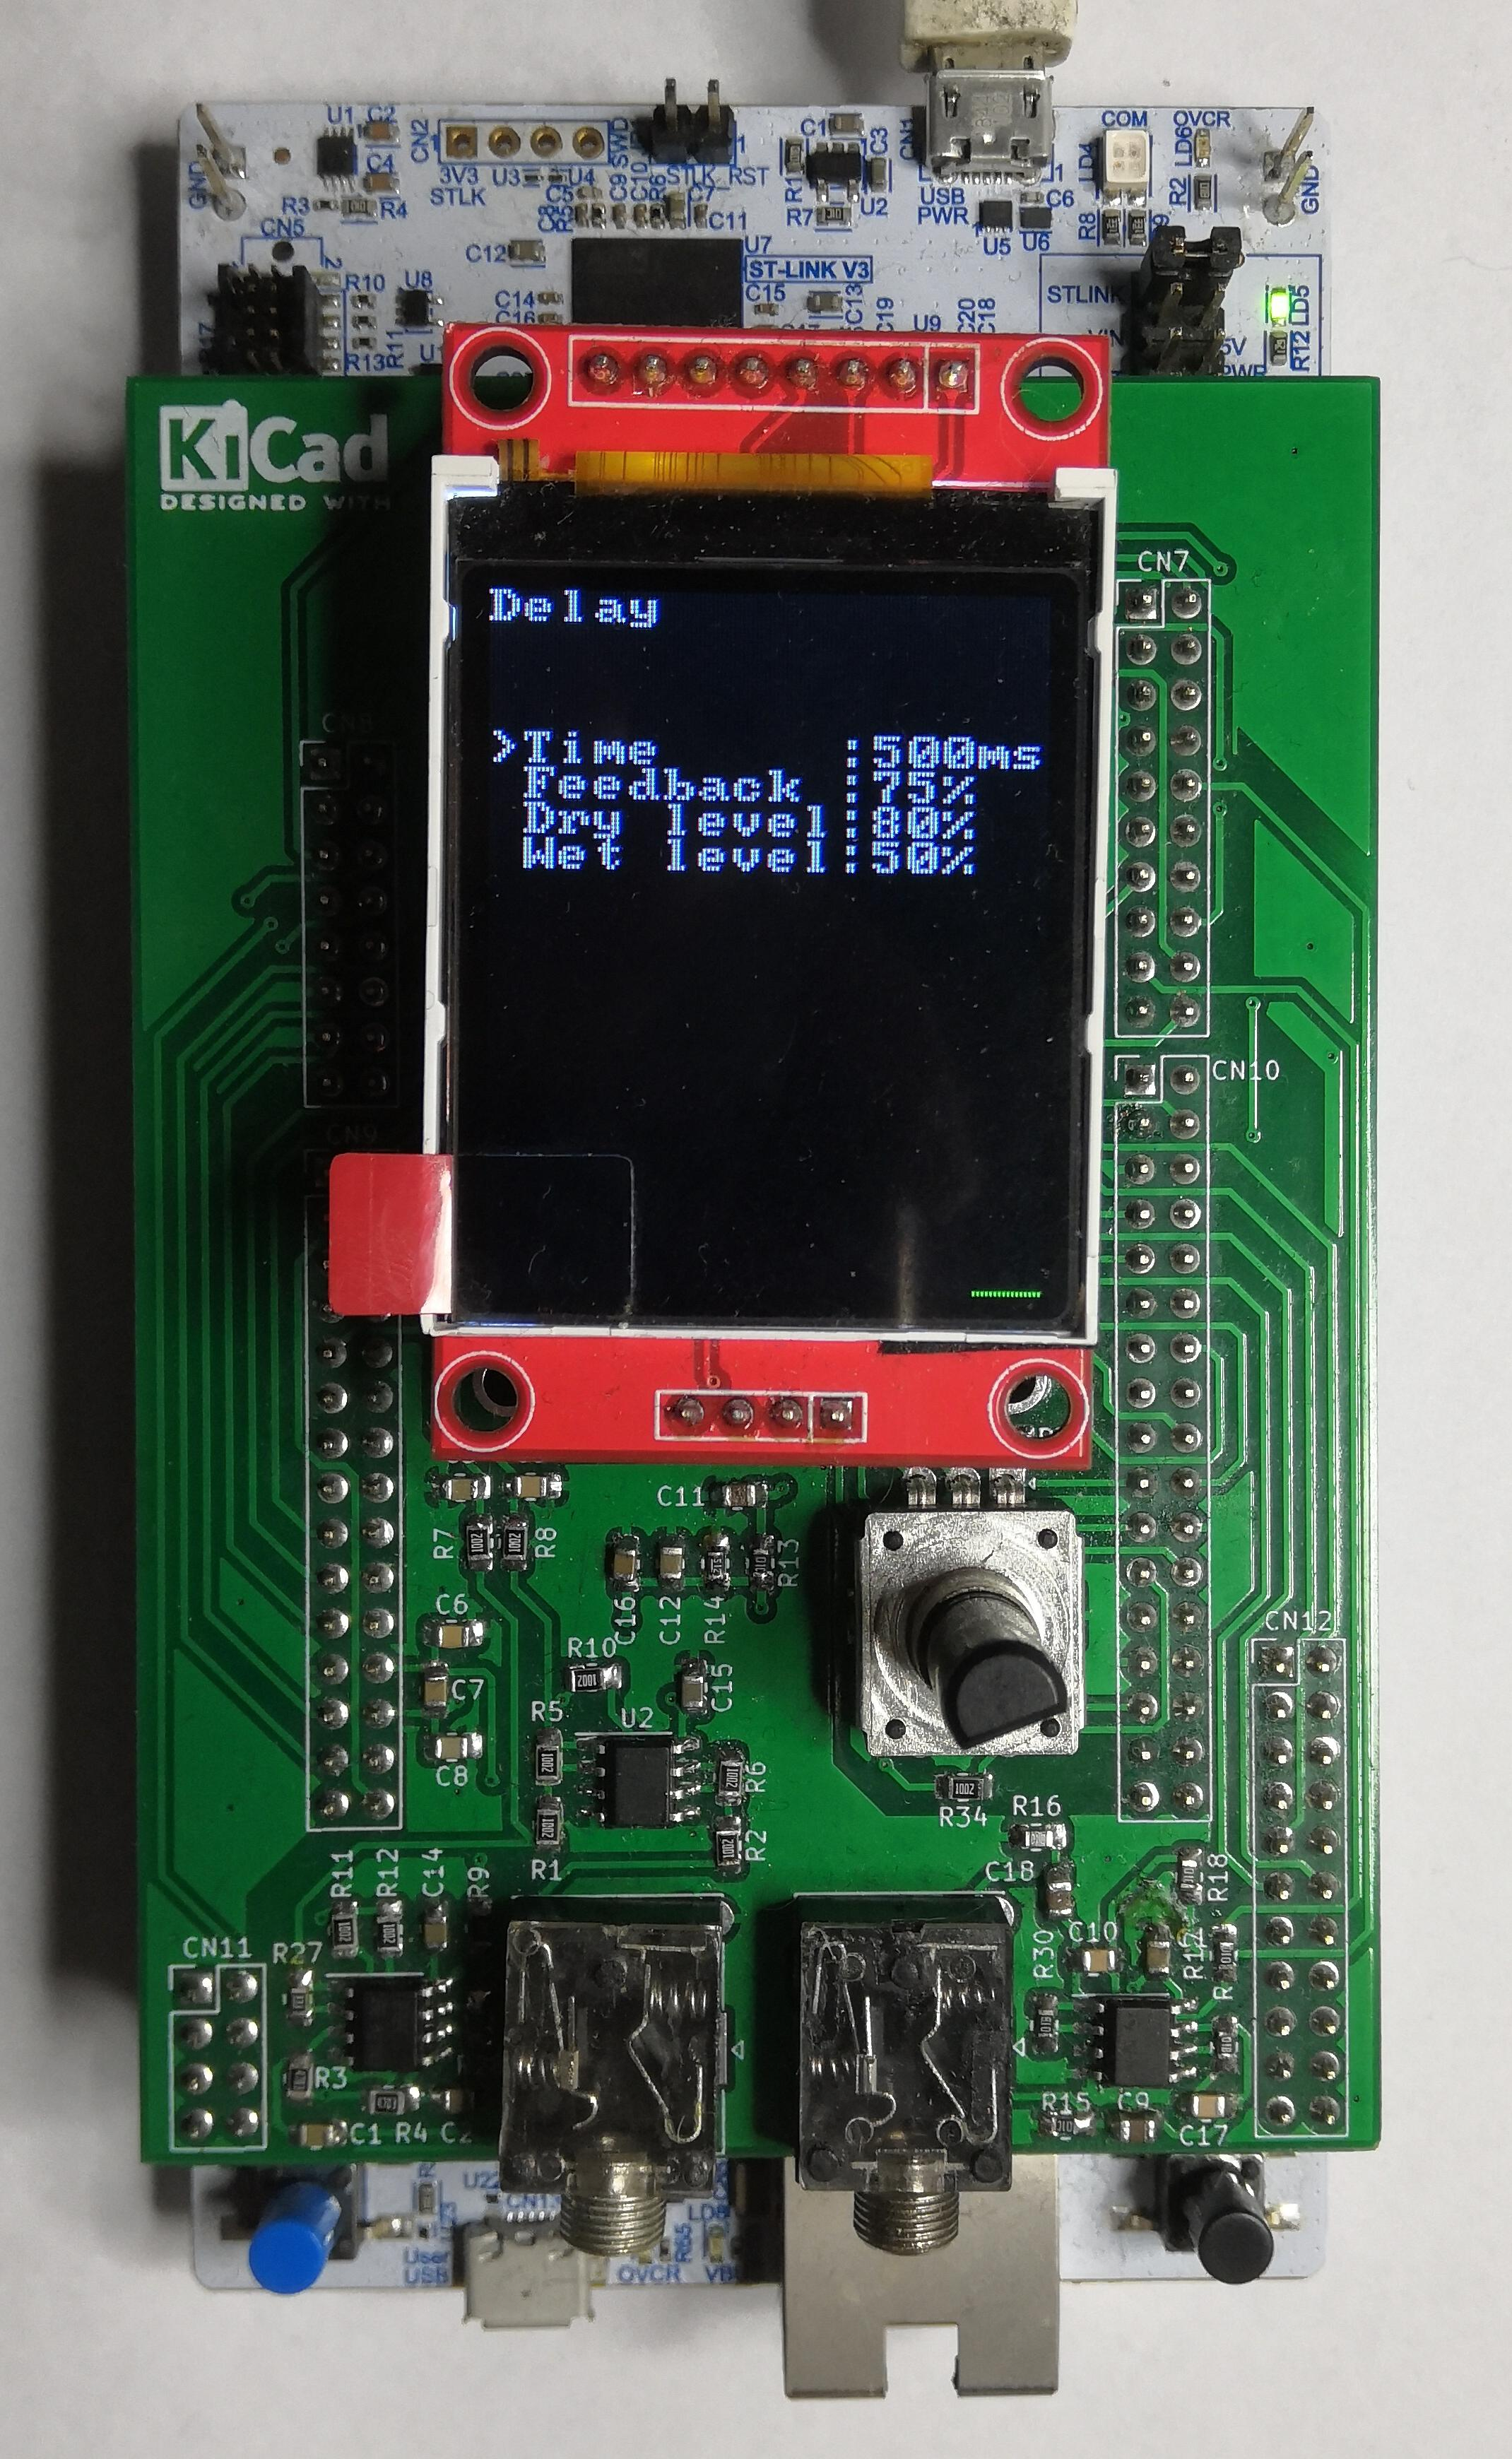
\includegraphics[angle=90,width=0.618\textwidth]{images/photo_working}
    \caption{Photo of the device during operation.}
    \label{fig:working}
\end{figure}

To use the device it must be connected to a power source.
It requires 5V to be applied through the top USB port,
which can be provided by micro USB smartphone charger,
powerbank or directly from computer.

The device has two mini jack connectors on the bottom of the board.
Connector on the left is analog output for the signal source.
It can be connected to line output of smartphone or computer sound card.
Right connector is analog output and should be connected
to an audio amplifier or active speakers.

While powered, the LCD screen should light up
and display white text on black background.
In the left top corner, name of currently selected effect is presented.
Below we can see a list of all parameters,
which can affect behavior of the effect.
On the right of each parameter, there is presented its current value.
On the left side, there is an arrow,
which purpose is to indicate currently selected parameter.

User can interract with device using rotary encoder
as well as black and blue buttons.
Rotating knob changes currently selected parameter.
To modify value of chosen parameter, user must push the encoder
to activate edit mode. It is indicated by green color of text.
In edit mode use can rotate knob to modify chosen value
and press it one more time to accept changes.

To change active effect, user must rotate the encoder
while blue button is depressed. User can also reset the device if needed.
To do it, user can press the black button,
which a hardware reset for both microcontroller and LCD screen.

Figure \ref{fig:screens} shows different screens
avaliable for corresponding effects.
On picture b) we can see, that one of the parameters is green.
It indicates, that parameter is in edit mode, as described previously.

\begin{figure}[H]
    \centering
    \begin{subfigure}[t]{0.23\textwidth}
        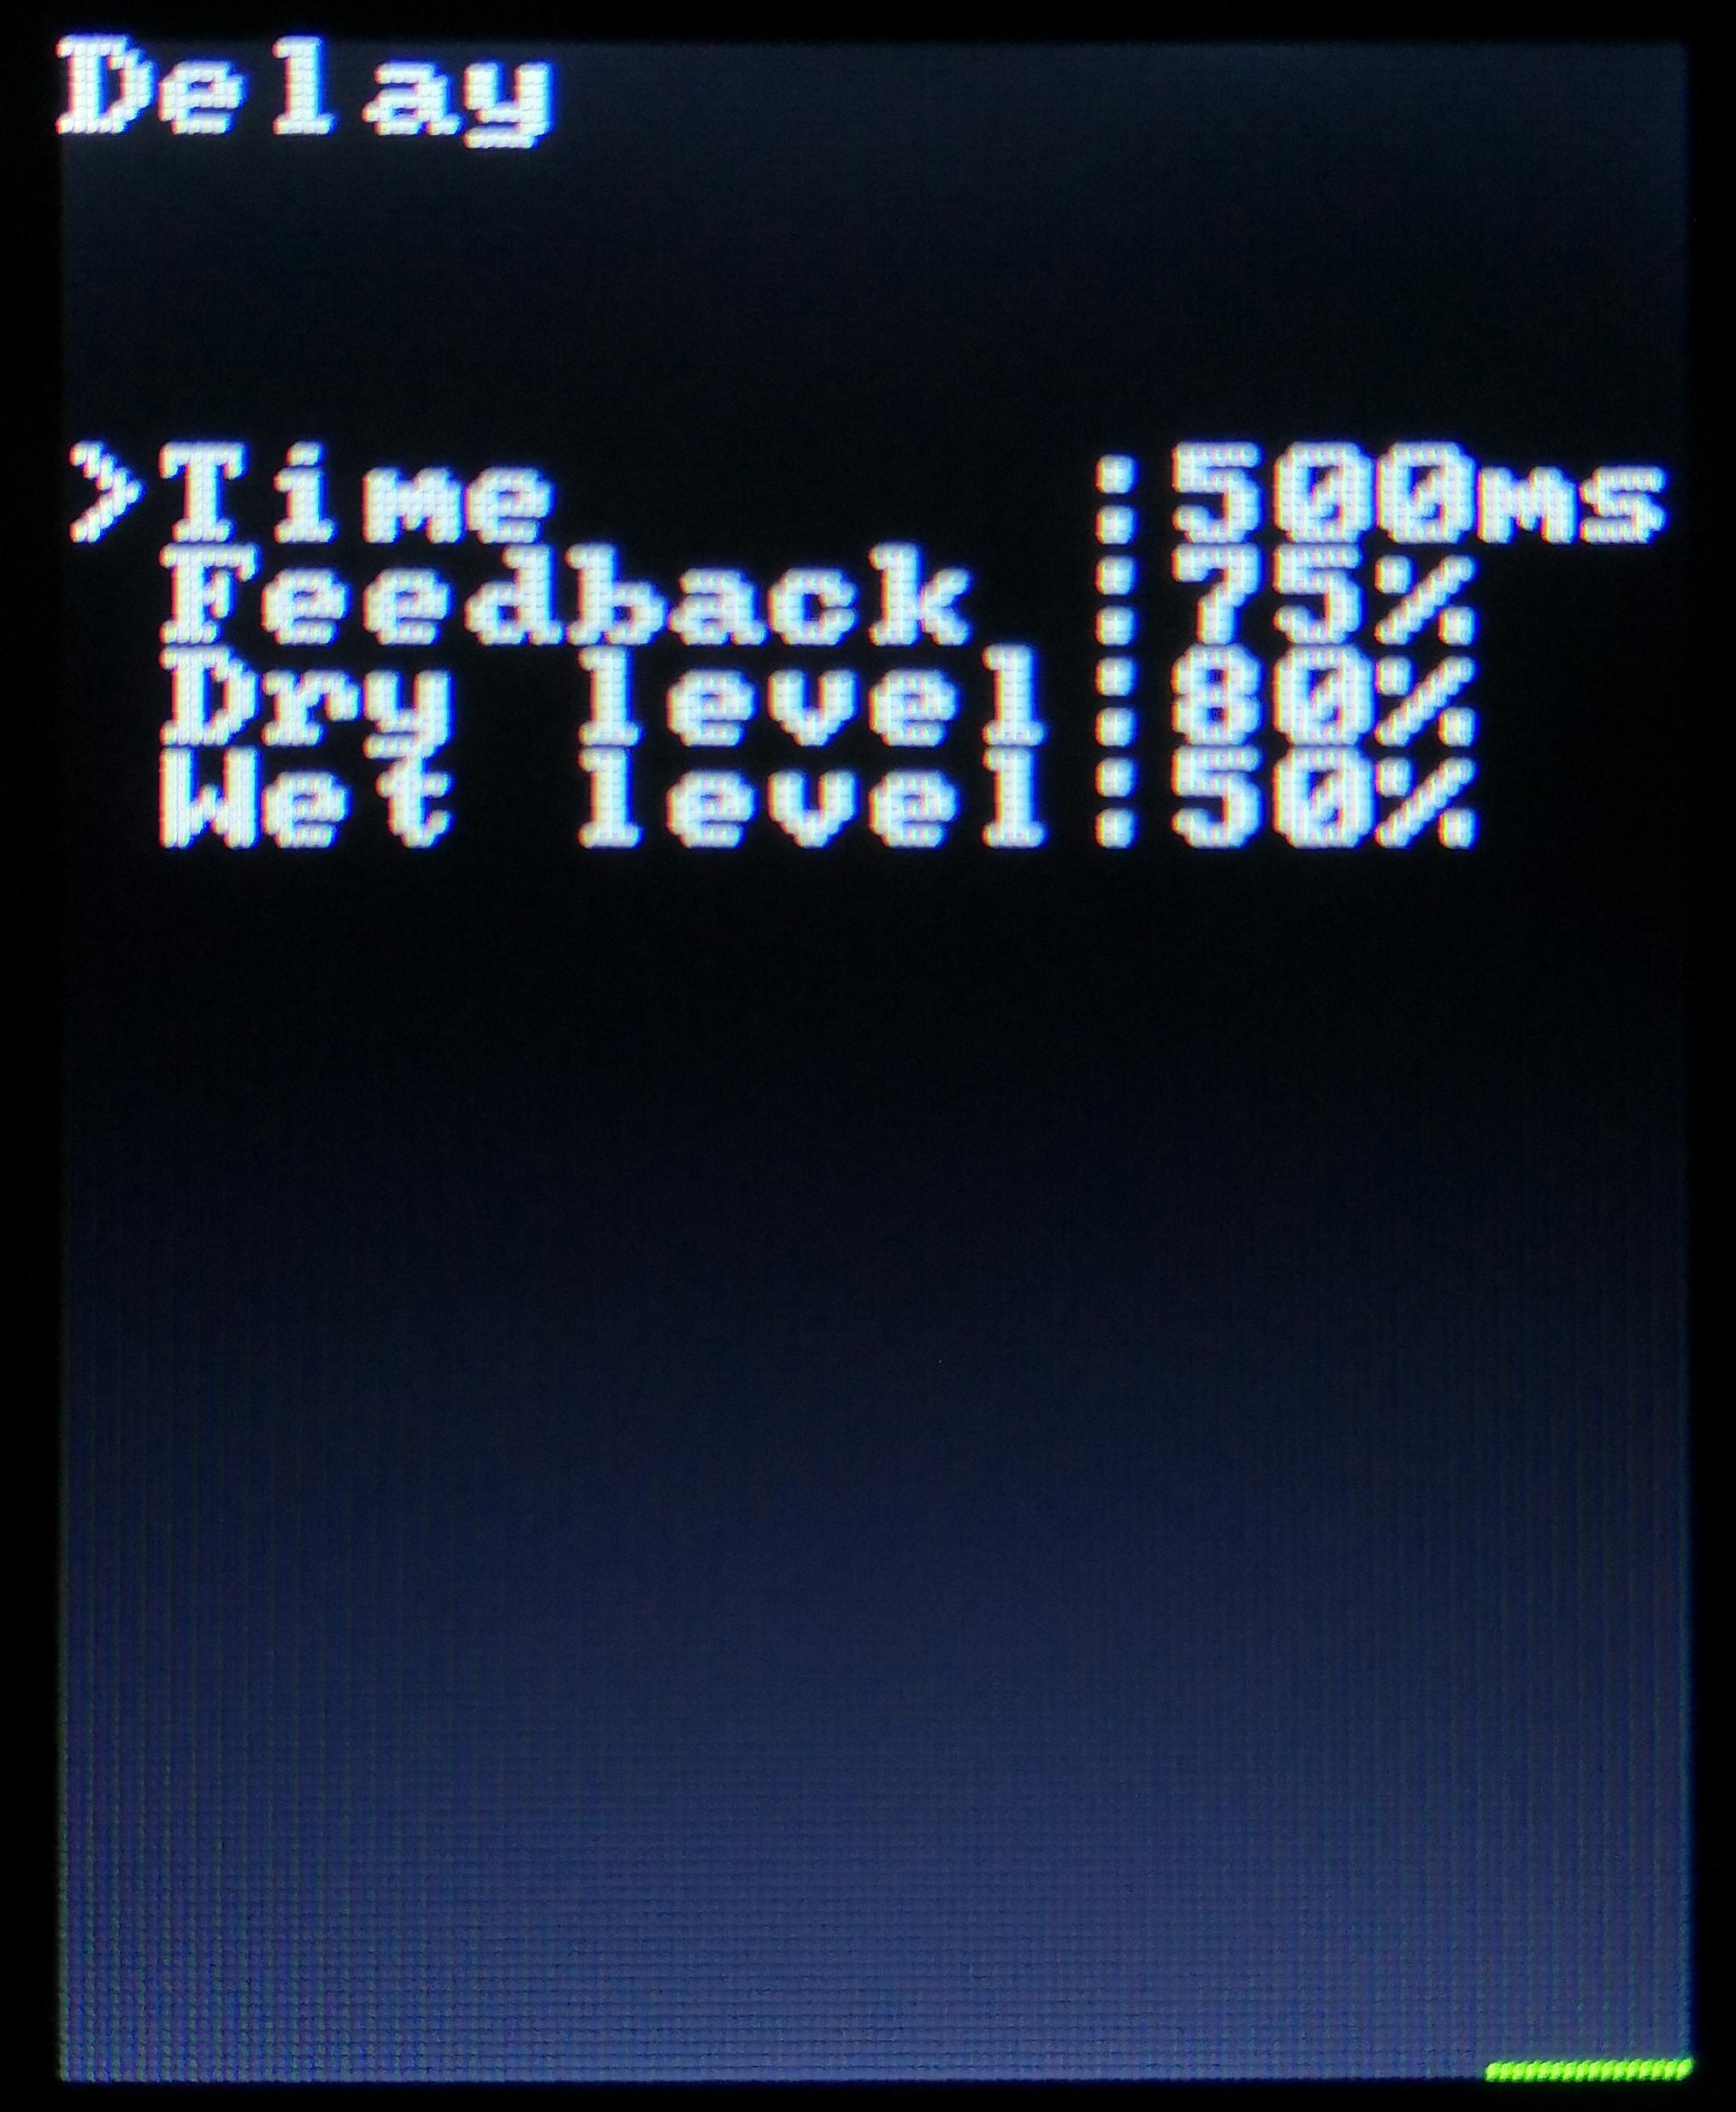
\includegraphics[width=\textwidth]{images/screen1}
        \caption{Delay screen.}
    \end{subfigure}
    ~
    \begin{subfigure}[t]{0.23\textwidth}
        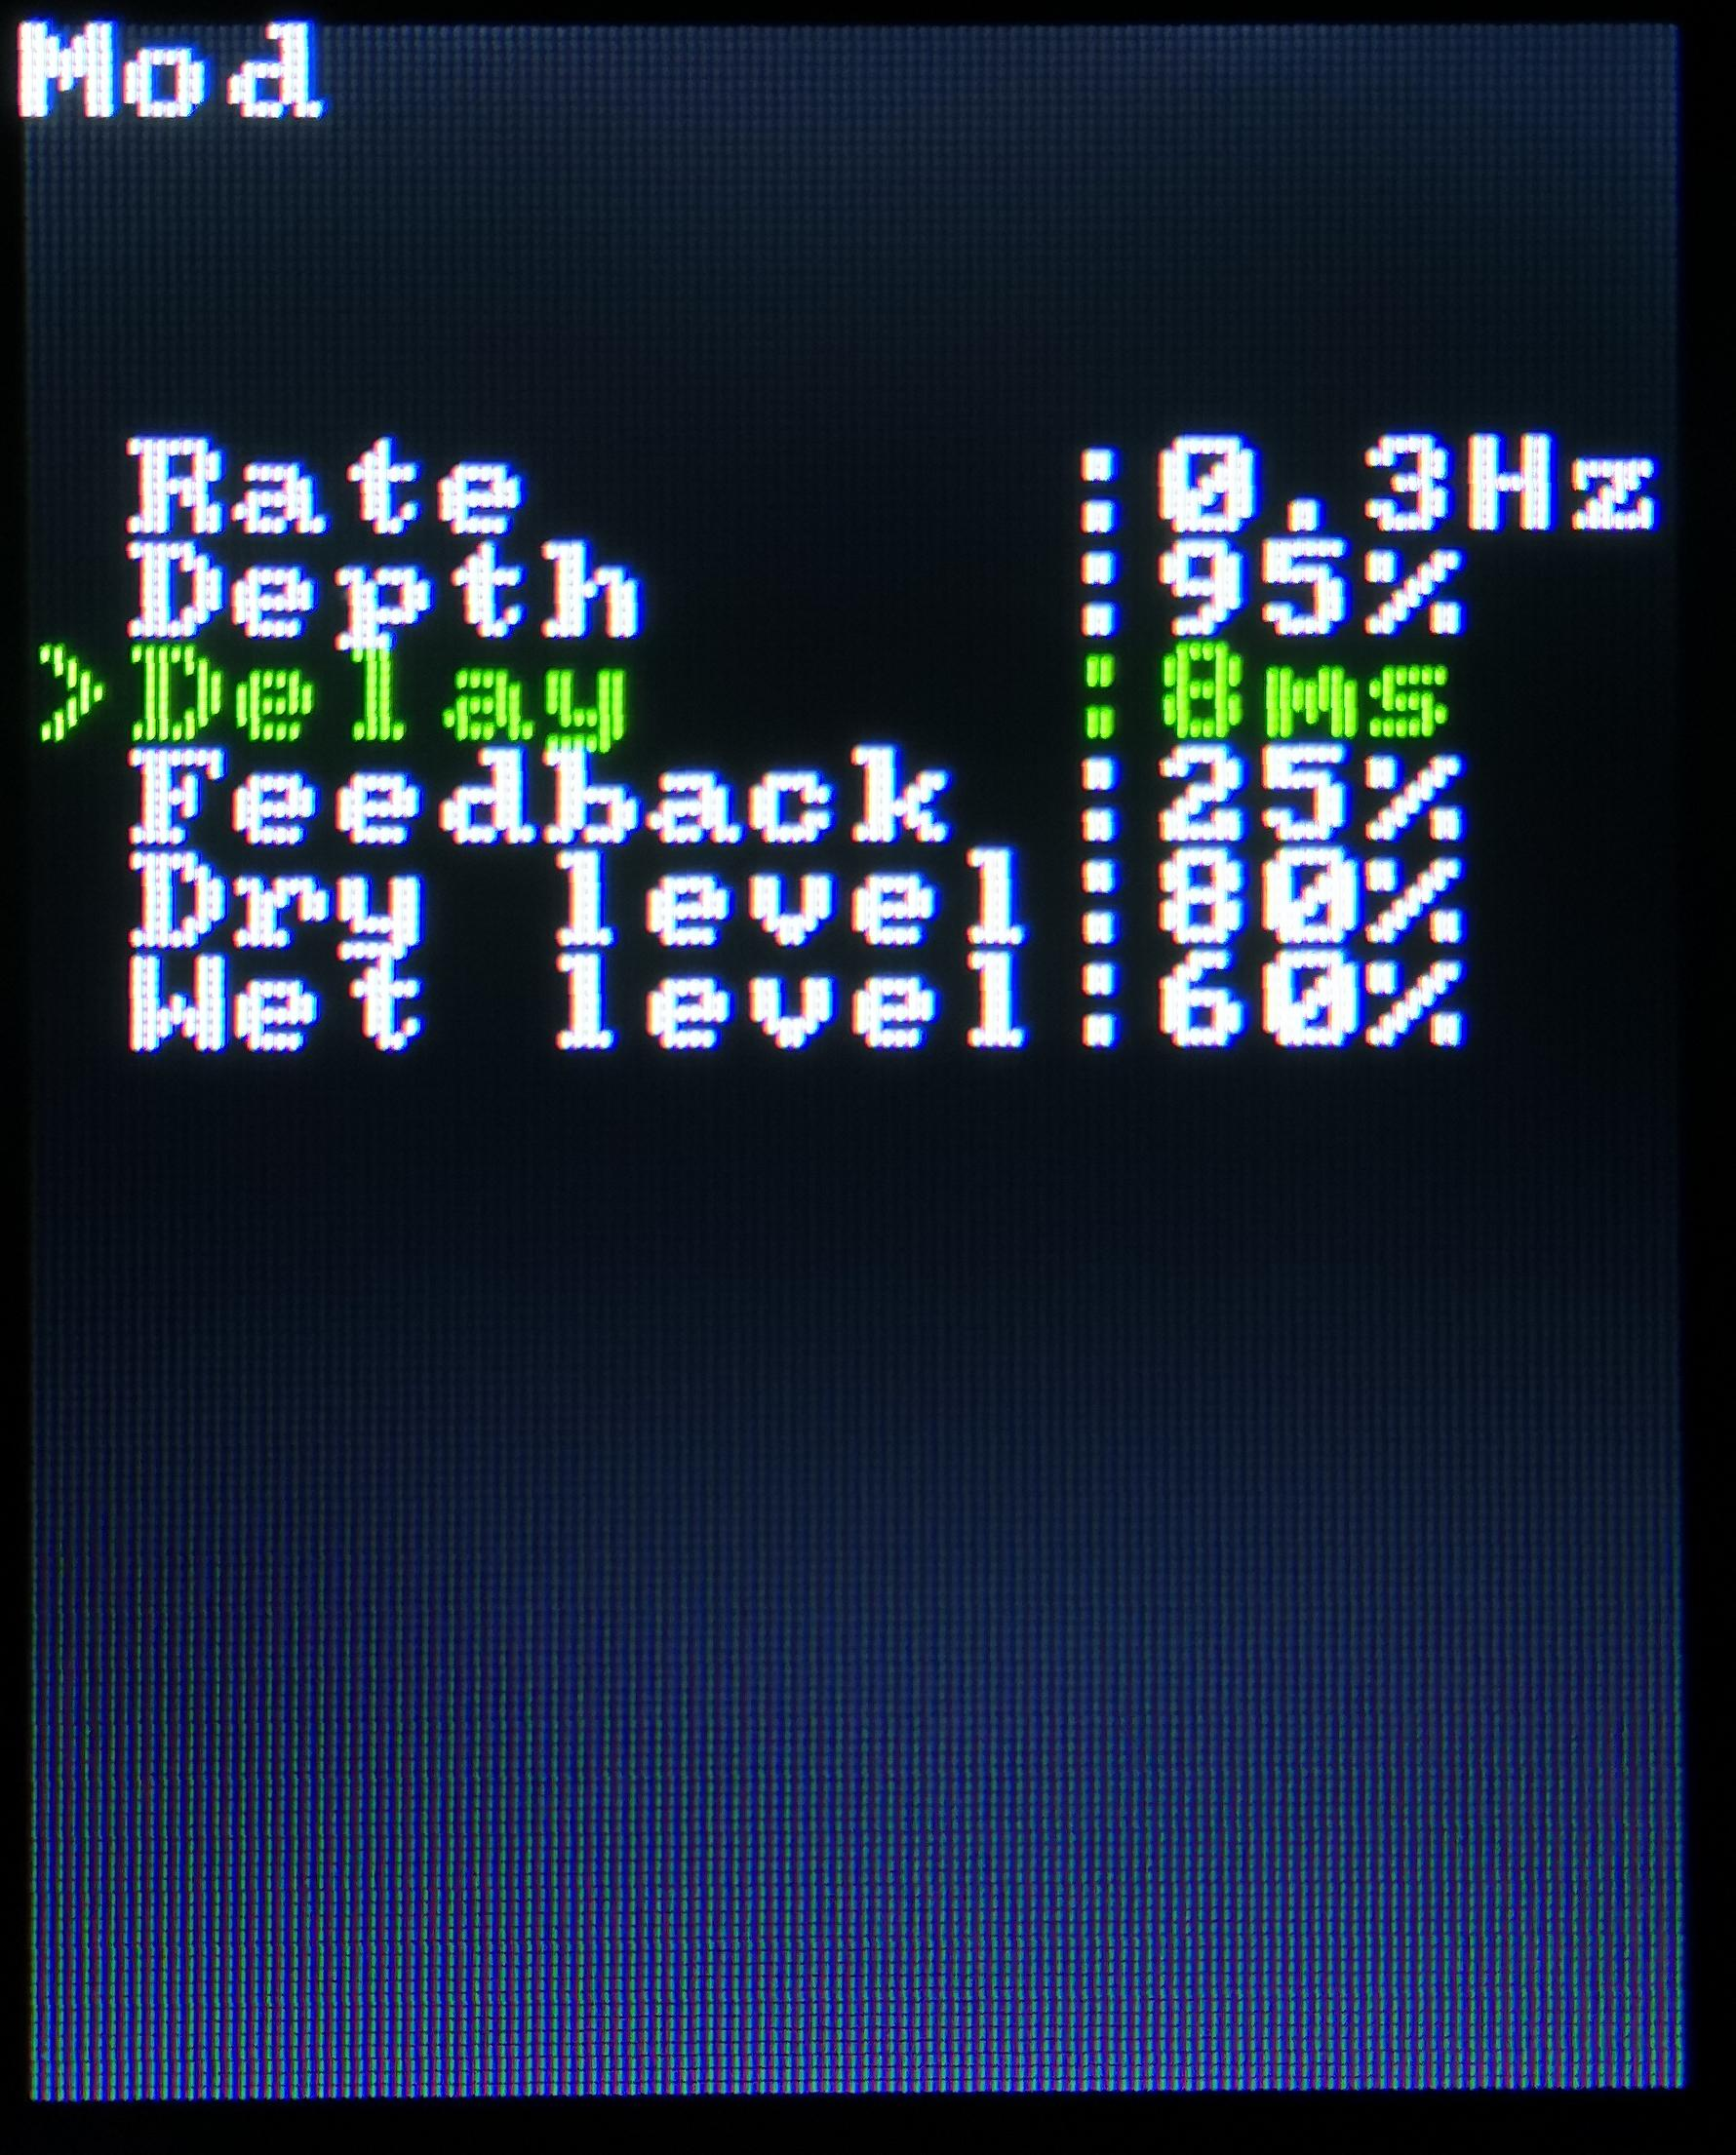
\includegraphics[width=\textwidth]{images/screen2}
        \caption{Modulation.}
    \end{subfigure}
    ~
    \begin{subfigure}[t]{0.23\textwidth}
        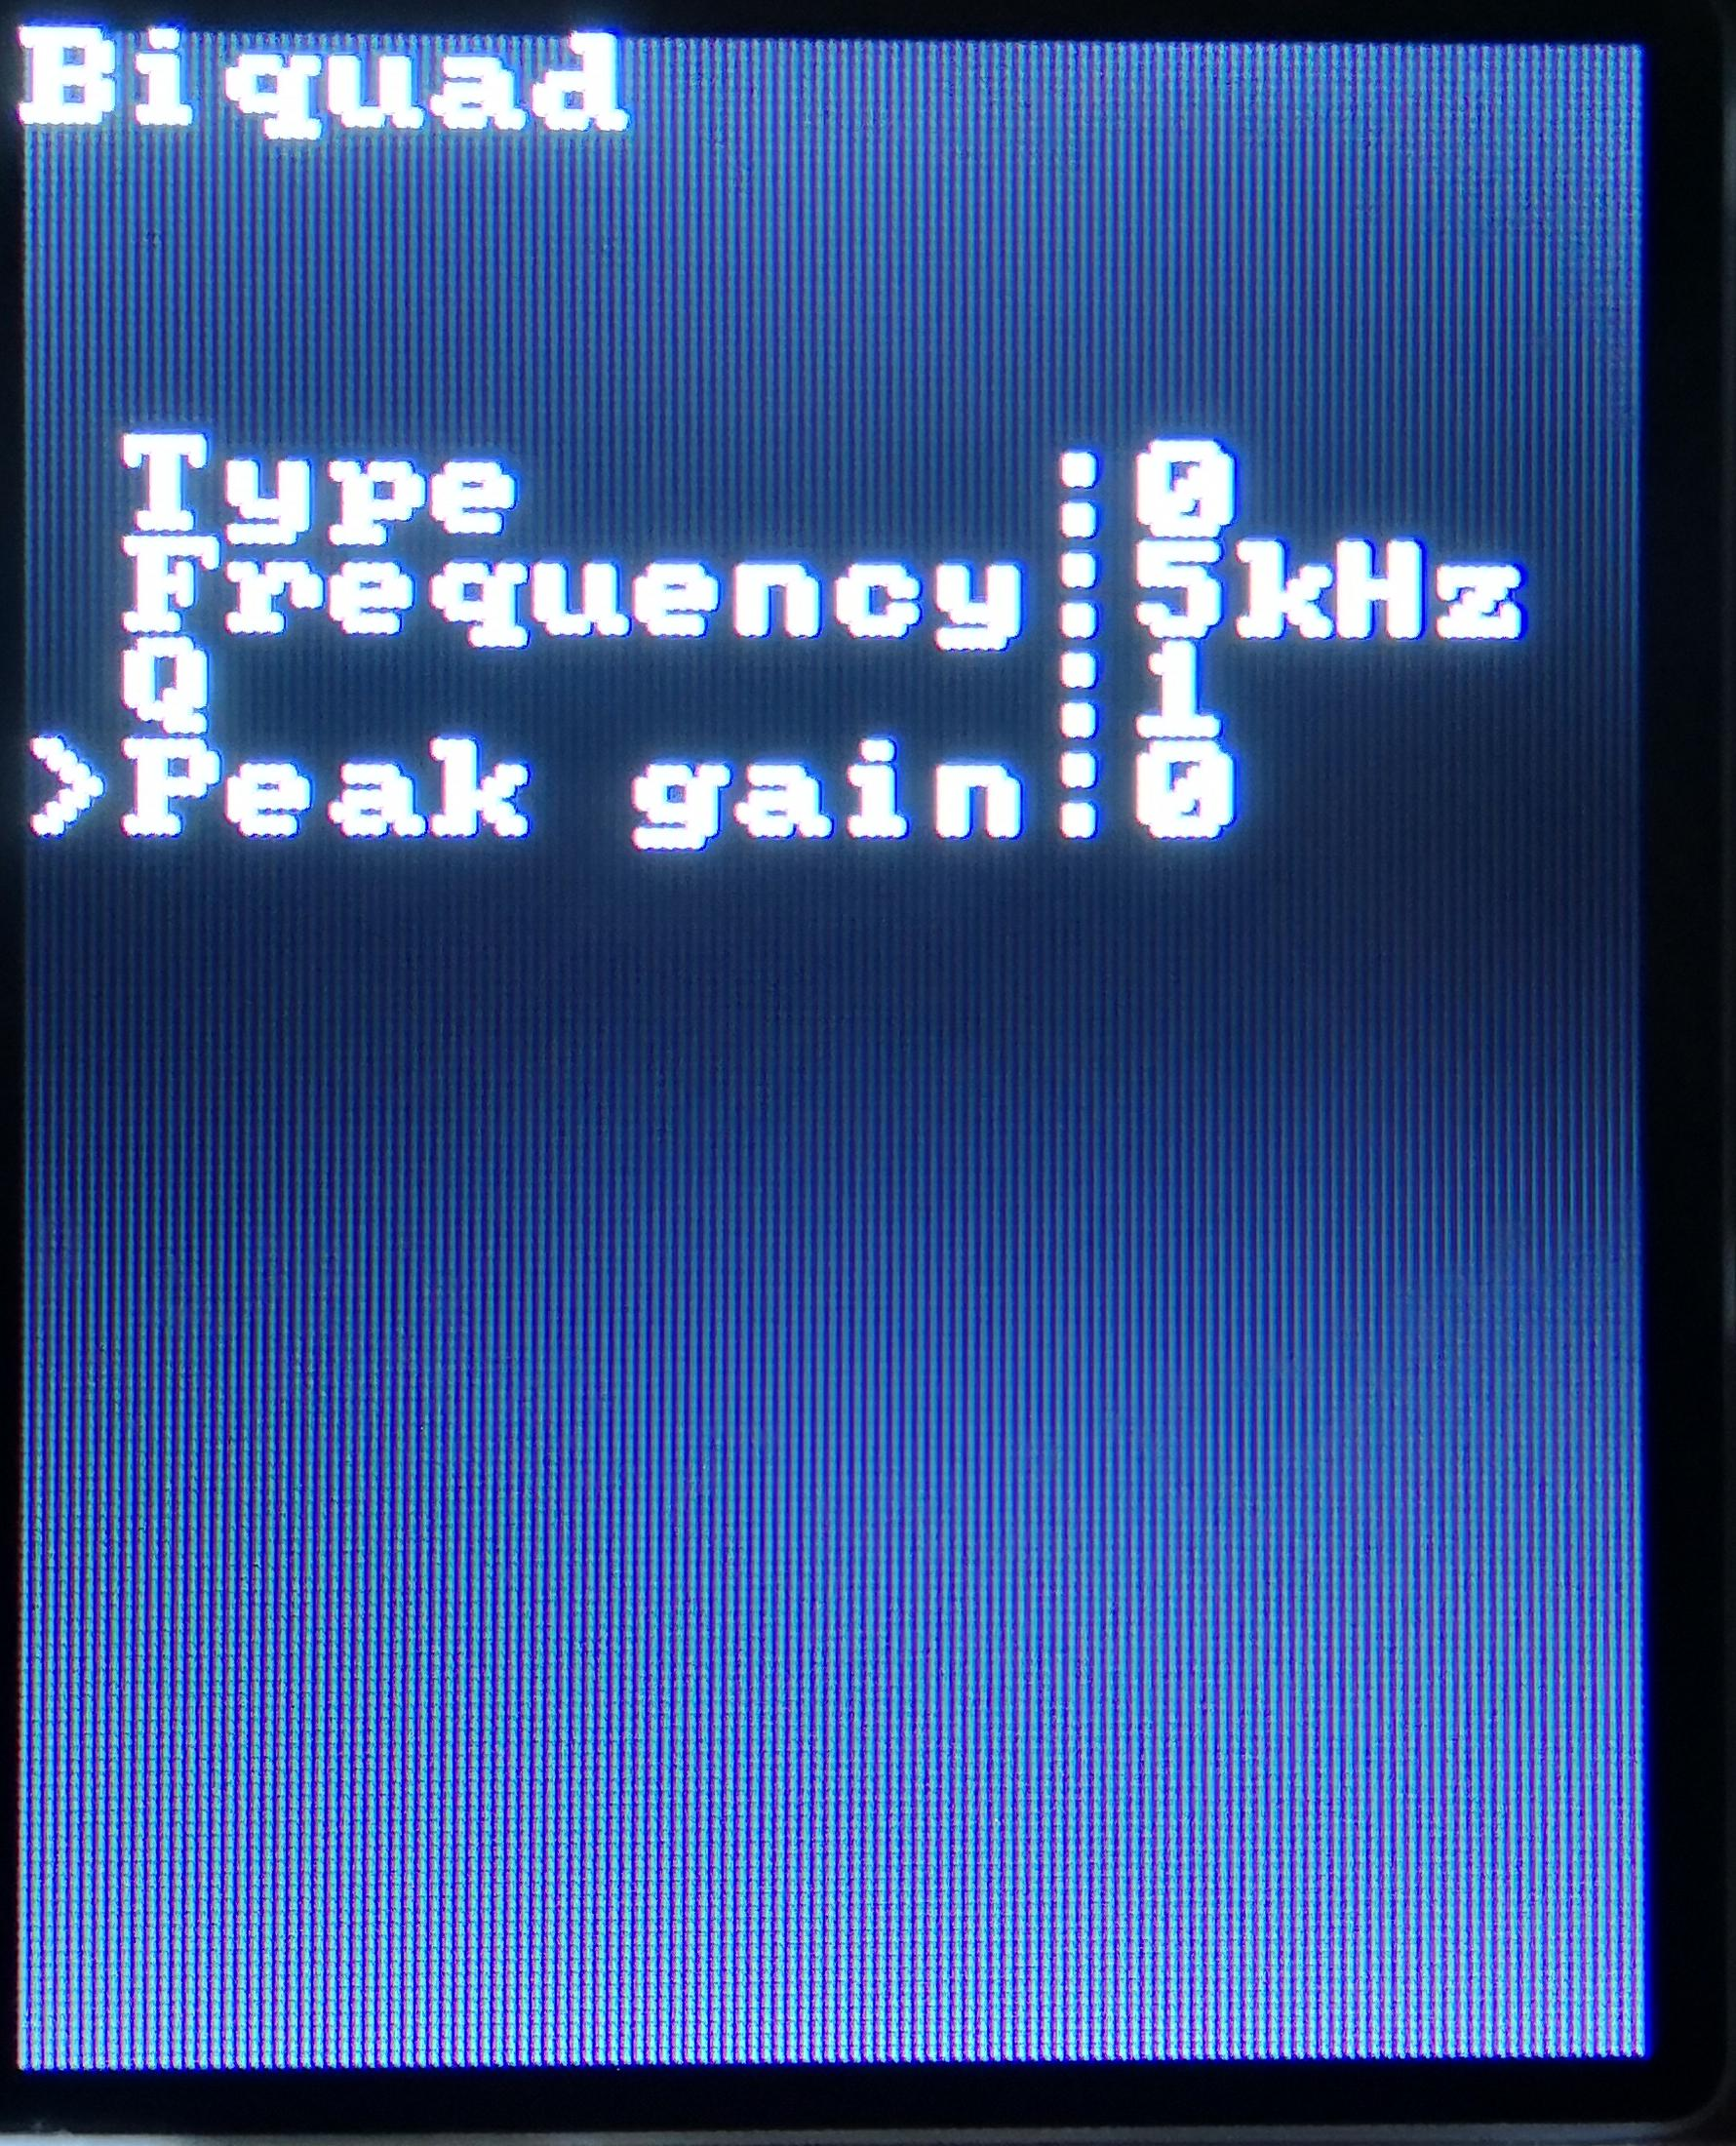
\includegraphics[width=\textwidth]{images/screen3}
        \caption{Biquad screen.}
    \end{subfigure}
    ~
    \begin{subfigure}[t]{0.23\textwidth}
        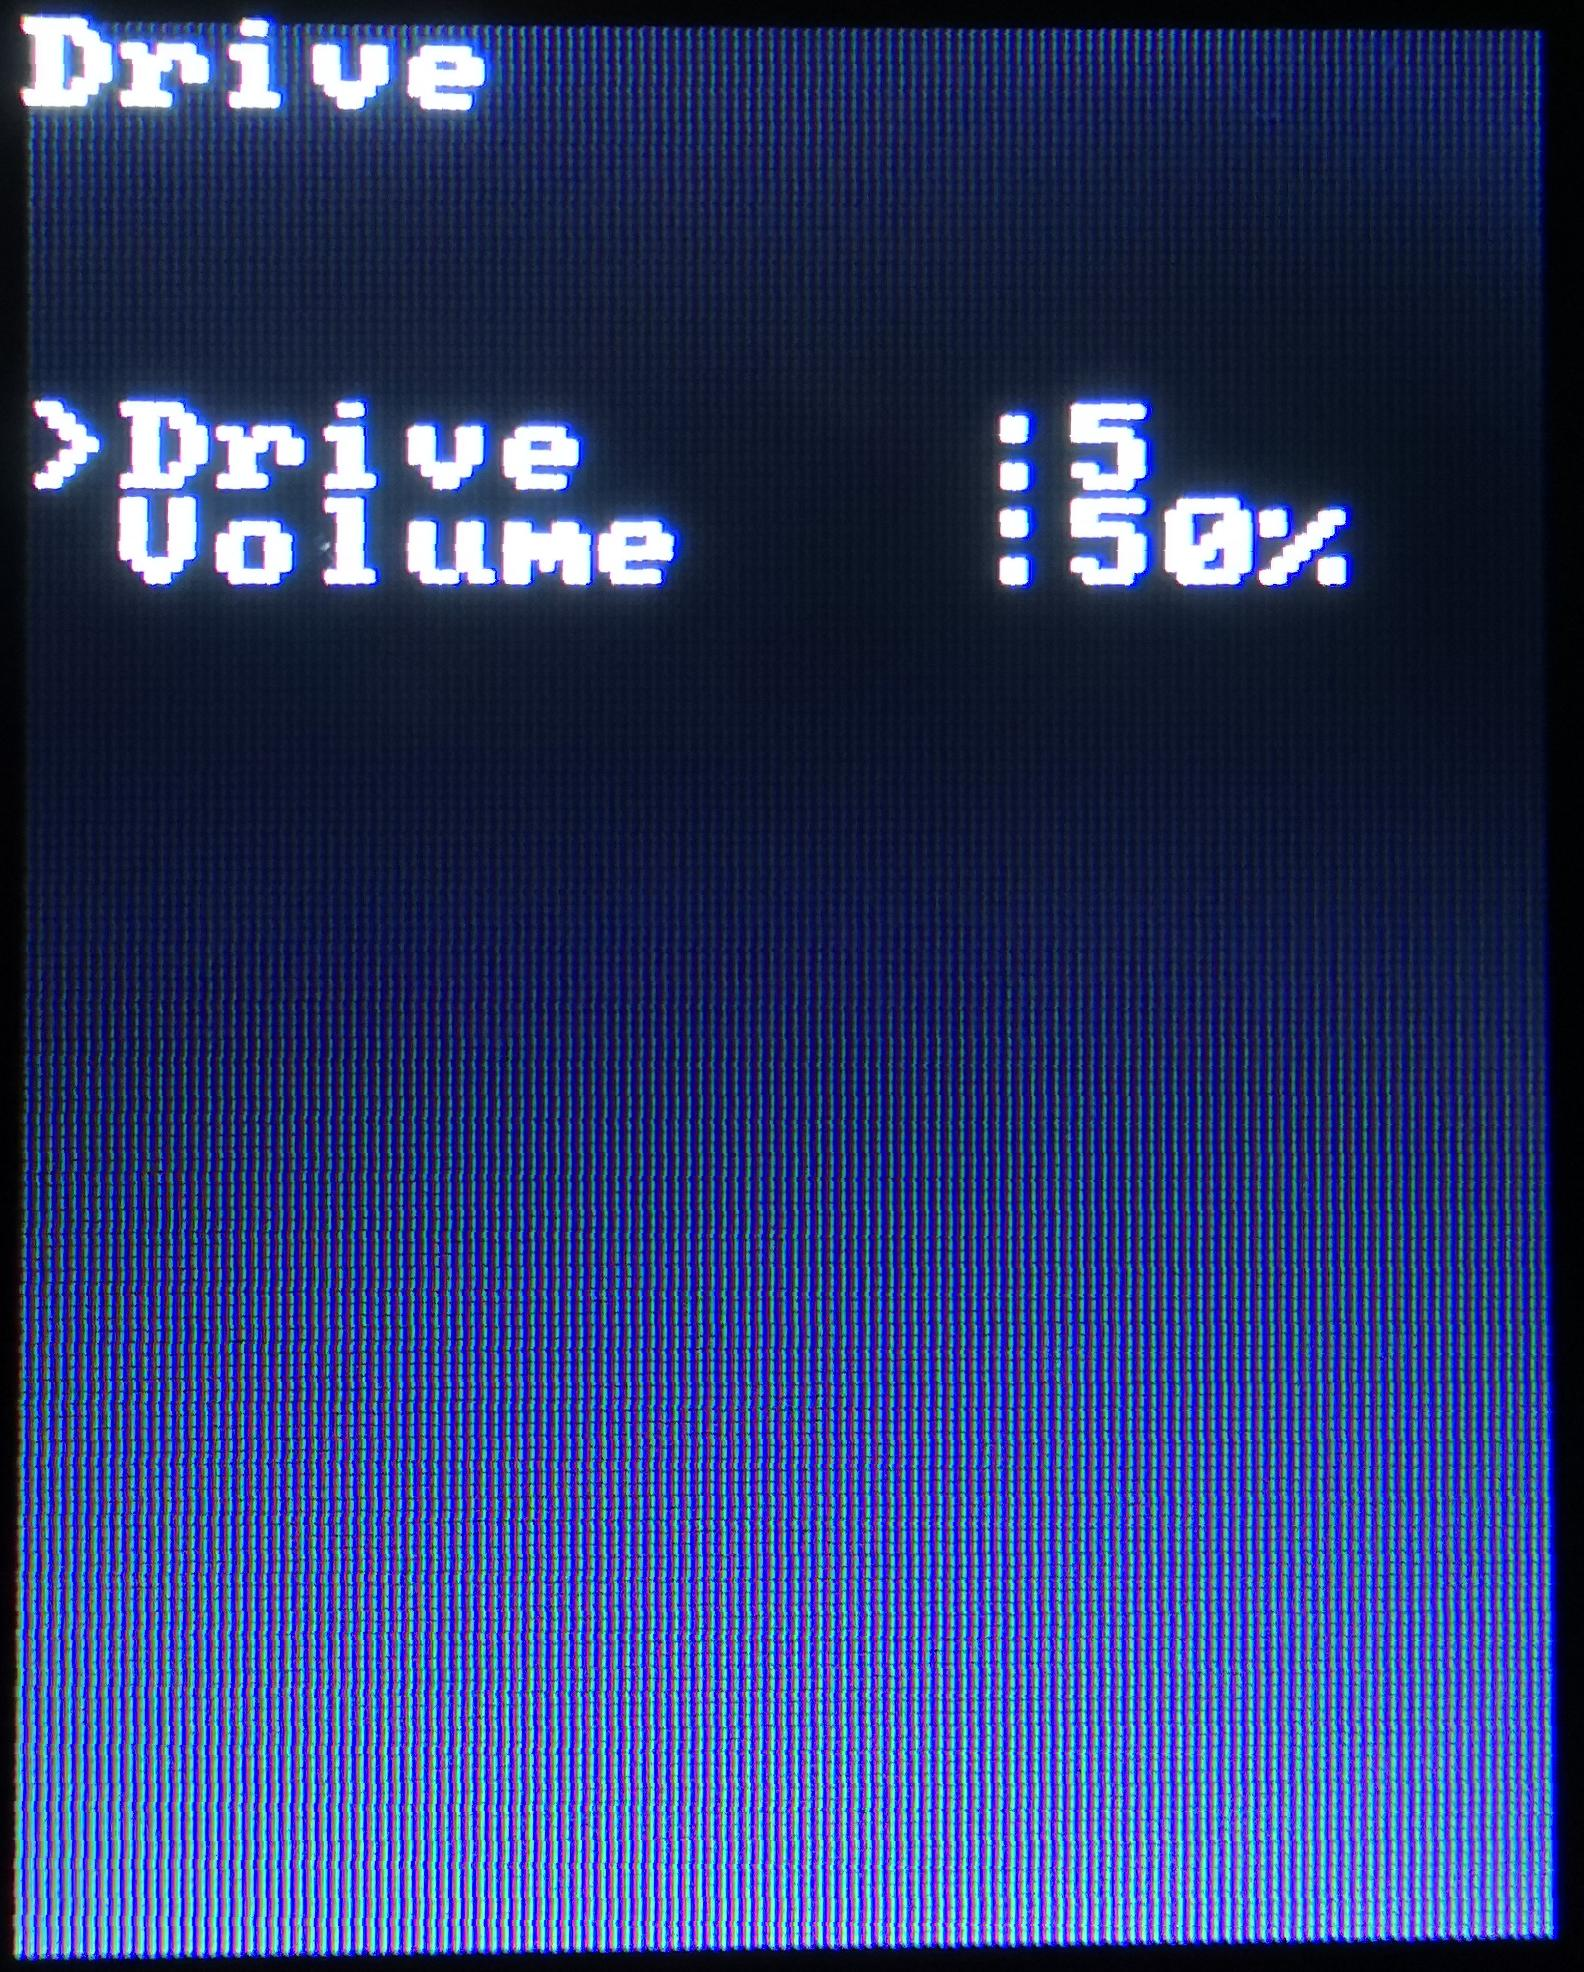
\includegraphics[width=\textwidth]{images/screen4}
        \caption{Drive screen.}
    \end{subfigure}
    \caption{Pictures of screen in different views.}
    \label{fig:screens}
\end{figure}

\chapter{Verification}\label{ch:verification}
This chapter is devoted to testing a device.
In following sections there ara timing diagrams and frequency
responses, which demonstrate working effects.

\section{Power consumption}
Power consumption was measured using a multimeter.
Nucleo board enables measurement of current,
by removing a JP2 jumper and plugging an ammeter in its place\cite{ST:UM2407}.
Using this method, current of 250mA was measured.
In combination with 5V supply voltage,
we obtain 1.25W of power consumption.

\section{Time diagrams}
Time diagrams were created using Audacity software and USB sound card.

\begin{itemize}
    \item Delay

    Figure \ref{fig:delay} presents timing diagram of delay effect.
    Part on the top shows input signal,
    which is an impulse generated with analog function generator.
    On the bottom of the picture, output of our device is presented.
    We can see fading reflections of the original signal.
    
    \begin{figure}[H]
        \centering
        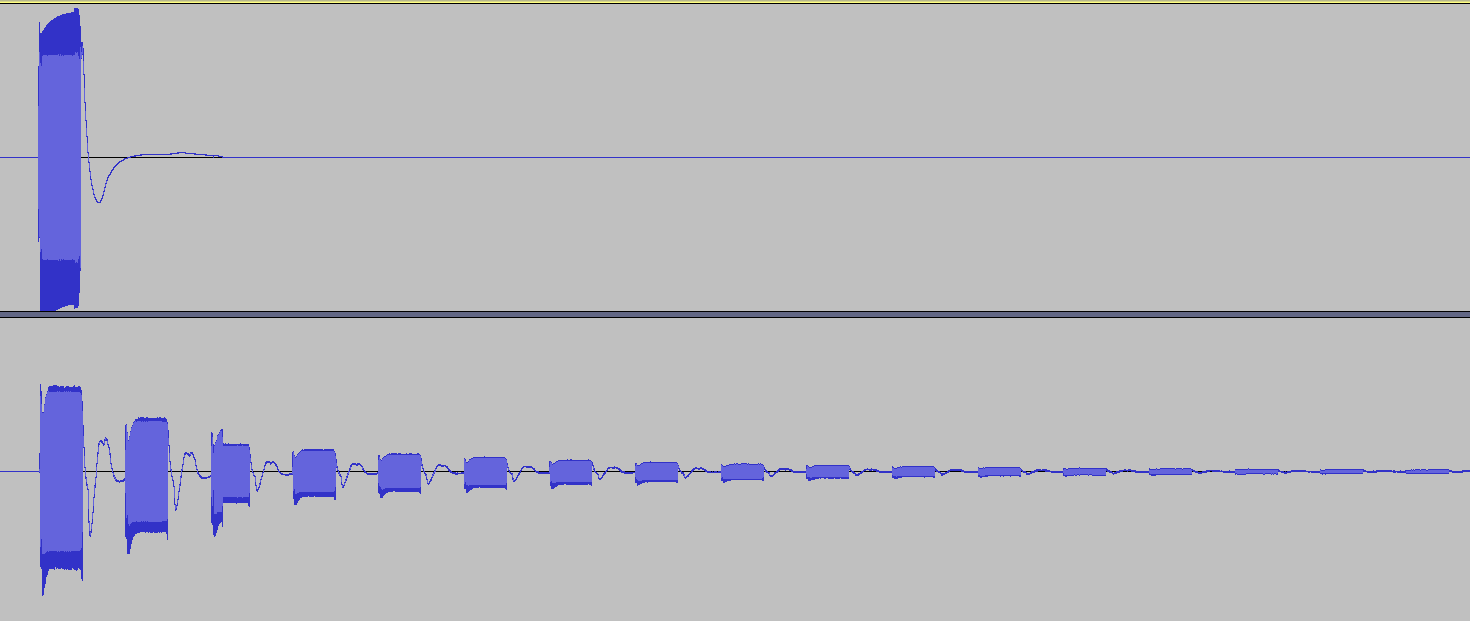
\includegraphics[width=0.95\textwidth]{images/delay}
        \caption{}
        \label{fig:delay}
    \end{figure}
    
    \item Modulation

    Timing diagram of modulation effect is presented at figure \ref{fig:mod}.
    Top part shows input signal, which is a 1kHz sine wave.
    Modulated signal can be seen at the bottom.
    Degradation of output signal is visible,
    which is caused by stretching signal in time.
    This problem could be resolved by using higher sampling frequency.

    \begin{figure}[H]
        \centering
        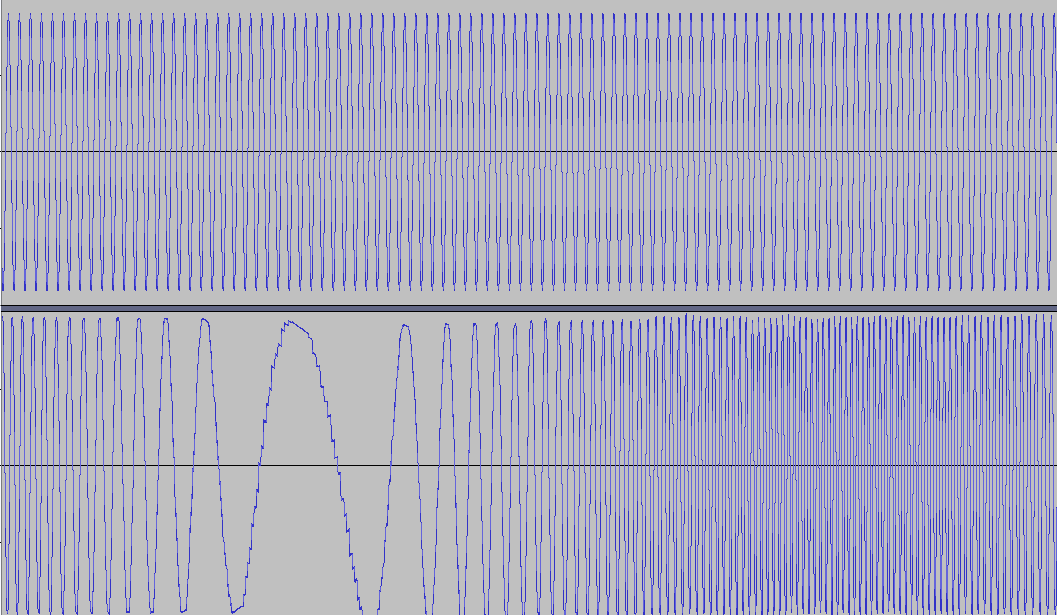
\includegraphics[width=0.95\textwidth]{images/modulation2}
        \caption{}
        \label{fig:mod}
    \end{figure}

    \item Drive
    Measurments of drive effect can be observed on figure \ref{fig:drive}.
    Peaks of input signal are flatened to produce harsh sound.
    
    \begin{figure}[H]
        \centering
        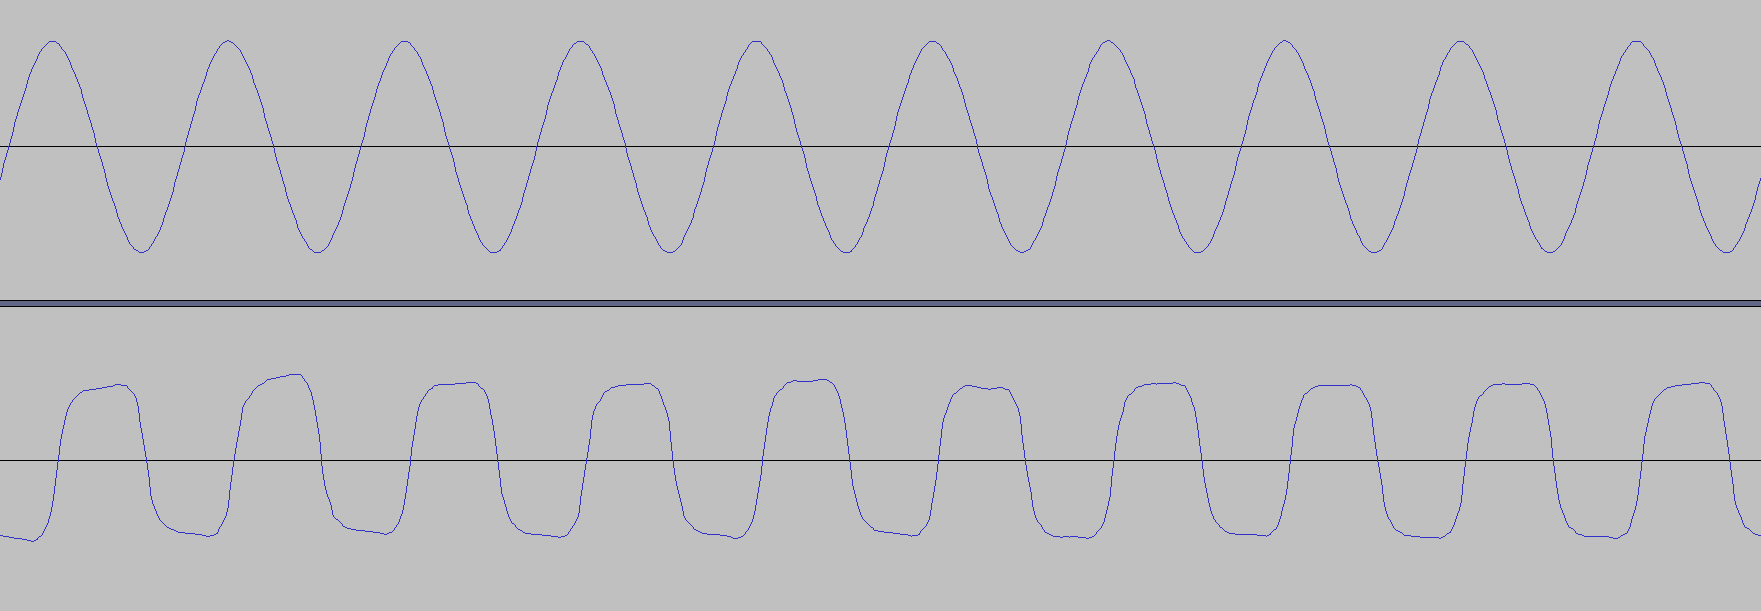
\includegraphics[width=0.95\textwidth]{images/drive}
        \caption{}
        \label{fig:drive}
    \end{figure}
\end{itemize}

\section{Characteristics}
Figure \ref{fig:filters} contains frequency response of different types of filters 
implemented using biquad algorithm.
RMAA 5.5 software was used to perform these measurements.
All filters have frequency set to 1kHz and Q-factor to 0.7.

\begin{figure}[h]
    \centering
    \begin{subfigure}[t]{0.45\textwidth}
        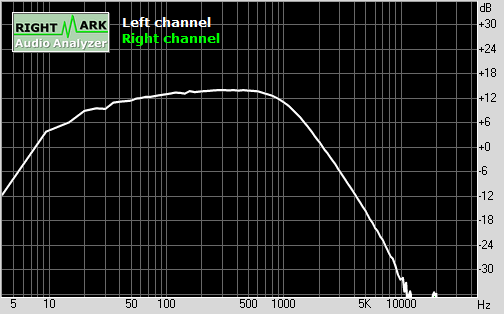
\includegraphics[width=\textwidth]{images/0_LPF}
        \caption{Low-pass filter.}
    \end{subfigure}
    ~
    \centering
    \begin{subfigure}[t]{0.45\textwidth}
        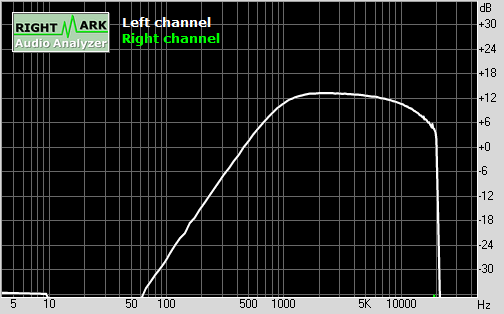
\includegraphics[width=\textwidth]{images/1_HPF}
        \caption{High-pass filter.}
    \end{subfigure}
    ~
    \centering
    \begin{subfigure}[t]{0.45\textwidth}
        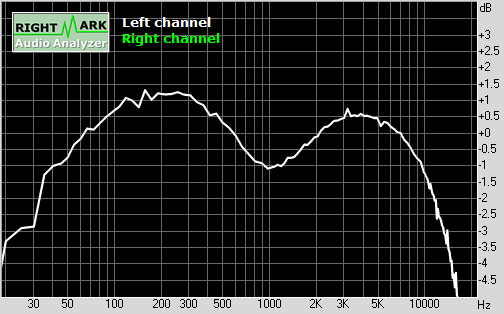
\includegraphics[width=\textwidth]{images/3_peak_minus3}
        \caption{Peak filter (-3dB).}
    \end{subfigure}
    ~
    \centering
    \begin{subfigure}[t]{0.45\textwidth}
        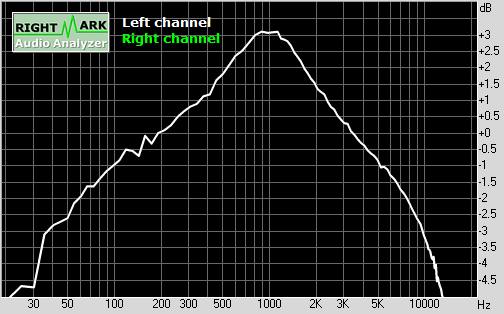
\includegraphics[width=\textwidth]{images/3_peak_plus3}
        \caption{Peak filter (+3dB).}
    \end{subfigure}
    ~
    \centering
    \begin{subfigure}[t]{0.45\textwidth}
        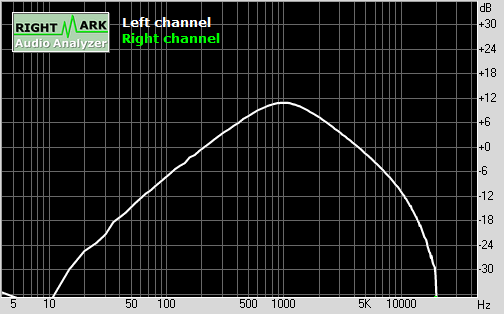
\includegraphics[width=\textwidth]{images/2_band}
        \caption{Band-pass filter.}
    \end{subfigure}
    ~
    \centering
    \begin{subfigure}[t]{0.45\textwidth}
        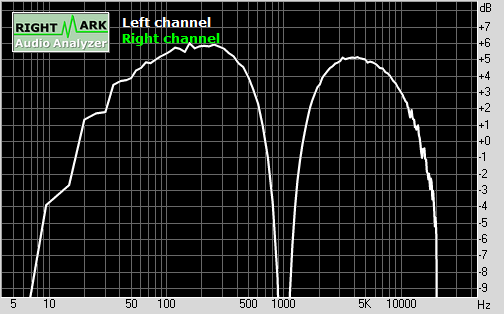
\includegraphics[width=\textwidth]{images/4_notch}
        \caption{Notch filter.}
    \end{subfigure}
    ~
    \centering
    \begin{subfigure}[t]{0.45\textwidth}
        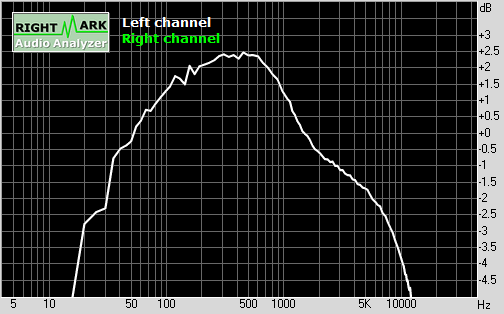
\includegraphics[width=\textwidth]{images/5_low}
        \caption{Low-shelf filter (+3dB).}
    \end{subfigure}
    ~
    \centering
    \begin{subfigure}[t]{0.45\textwidth}
        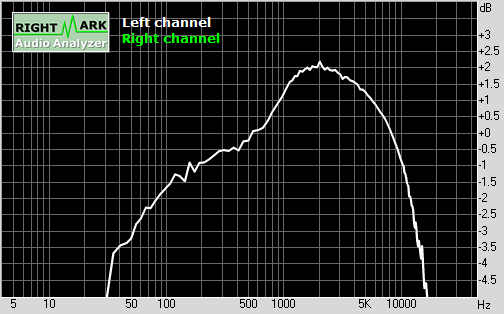
\includegraphics[width=\textwidth]{images/6_high}
        \caption{High-shelf filter (+3dB).}
    \end{subfigure}
    \caption{Measured frequency responses.}
    \label{fig:filters}
\end{figure}

\section{Recordings}
Attached CD contain audio files,
which present how different effects sound.

\chapter{Summary}\label{ch:summary}
All goals and tasks of the projects were accomplished.
Process involved different aspects of technology.
One of was them creation of schematic and board layout,
which are only the first step necessary to obtain 
the physical layer of the device.
The next step was whole manufacturing process.
Fortunately PCB manufacturers provide great support
and require only gerber files to create a board.
Last step to create a device was assembly,
which required some manual skills.

Creating software requires completely different
knowledge and skills than all previous steps.
Understanding of Arm architecture was necessary
to select proper tools and configure device properly.
Experience with object oriented programming
allowed to create very modular and easy to modify program.

Whole project was very educational.
It required reading user manuals and datasheets of particular components
in order to obtain desired results.
Developing software involved some debugging,
which was simplified thanks to selected tools.

The project is very flexible and has some room for potential expansion.
There is still free memory to implement new effect, more complex UI,
and more features such as casscading effects.

%%%%%%%%%%%%%%%%%%%%%%%%%%%%%%%%%%%%%%%%%%
\backmatter
\pagenumbering{Roman}
\stepcounter{PagesWithoutNumbers}
\setcounter{page}{\value{PagesWithoutNumbers}}

\pagestyle{onlyPageNumbers}

%%%%%%%%%%% bibliography %%%%%%%%%%%%
\printbibliography

%%%%%%%%%  appendices %%%%%%%%%%%%%%%%%%% 

% \begin{appendices} 

% \chapter*{List of abbreviations and symbols}

% \begin{itemize}
% \item[ADC] - Analog to digital converter
% \item[API] - Application programming interface
% \item[CPU] - Central processing unit
% \item[DAC] - Digital to analog converter
% \item[DC] - Direct current
% \item[DMA] - Direct memory access
% \item[DSP] - Digital signal processing
% \item[EDA] - Electronic design automation
% \item[FFT] - Fast fourier transform
% \item[FMC] - Flexible momory controller
% \item[FPU] - Floating-point uint
% \item[GCC] - GNU Compiler Collection
% \item[GPIO] - General purpose input/output
% \item[IDE] - Integrated development environment
% \item[IIR] - Infinite impulse response
% \item[LCD] - Liquid crystal display
% \item[LFO] - Low frequency oscillator
% \item[LQFP] - Low-profile quad flat pack
% \item[MCU] - Microcontroller Unit
% \item[PCB] - Printed circuit board
% \item[RAM] - Random access memory
% \item[ROM] - Read only memory
% \item[SDRAM] - Synchronous dynamic random access memory
% \item[SMD] - Surface mounted device
% \item[SOIC] - Small outline integrated circuit
% \item[SPI] - Serial peripheral interface
% \item[UI] - User interface
% \end{itemize}

\chapter*{Contents of attached CD}

The thesis is accompanied by a CD containing:
\begin{itemize}
\item thesis (\LaTeX\ source files and final \texttt{pdf} file),
\item source code of the application,
\item schematic and board layout (KiCad, \texttt{pdf} and gerber files),
\item audio recording:w
 presenting selected effects
\end{itemize}

% \listoffigures

% \end{appendices}

\end{document}
